% ============================================================
% MSAS-GNN 硕士学位论文答辩 Beamer 演示文稿
% 北京师范大学 统计学院
% ============================================================
\documentclass[aspectratio=169,9pt,xcolor=dvipsnames]{beamer}
\usetheme{default}
\usecolortheme{default}

% ---------- 中文支持 ----------
\usepackage{xeCJK}
\setCJKmainfont[BoldFont={* Bold}]{Kaiti SC}
\setCJKsansfont[BoldFont={* Bold}]{Kaiti SC}
\setCJKmonofont[BoldFont={* Bold}]{Kaiti SC}

% ---------- 英文字体 ----------
\setmainfont{Times New Roman}
\setsansfont{Times New Roman}

% ---------- 数学与符号 ----------
\usepackage{amsmath,amssymb,amsthm}
\usepackage{algpseudocode}
\usepackage{mathrsfs}
\usepackage{bm}
\usepackage{bbm}

% ---------- 图表 ----------
\usepackage{graphicx}
\usepackage{tikz}
\usetikzlibrary{shapes,arrows,positioning,calc}
\usepackage{pgfplots}
\pgfplotsset{compat=1.18}

% ---------- 表格 ----------
\usepackage{booktabs}
\usepackage{multirow}
\usepackage{array}

% ---------- 其他 ----------
\usepackage{hyperref}
\usepackage{xcolor}

% ==================== 颜色定义 ====================
\definecolor{mynavy}{RGB}{37,62,112}
\definecolor{myred}{RGB}{192,64,64}
\definecolor{mygreen}{RGB}{26,144,112}

% ==================== 自定义命令 ====================
\newcommand{\highlight}[1]{\textcolor{myred}{\textbf{#1}}}
\newcommand{\blue}[1]{\textcolor{mynavy}{#1}}
\newcommand{\green}[1]{\textcolor{mygreen}{#1}}
\newcommand{\kbar}{\ensuremath{\bar{k}}}

% ==================== 章节角标（TikZ overlay，不影响版式） ====================
\newcommand{\chapternote}{}
\newif\ifshowchapternote
\showchapternotefalse
\newcommand{\setchapternote}[1]{%
  \renewcommand{\chapternote}{#1}%
  \showchapternotetrue
}
\addtobeamertemplate{headline}{}{%
  \ifshowchapternote
  \begin{tikzpicture}[remember picture, overlay]
    \node[anchor=north east, fill=mynavy!15, draw=mynavy!60,
          rounded corners=3pt, inner sep=4pt,
          font=\footnotesize\bfseries\color{mynavy}]
      at ([xshift=-6pt, yshift=-6pt] current page.north east) {\chapternote};
  \end{tikzpicture}%
  \fi
}

\renewcommand{\algorithmicrequire}{\textbf{输入：}\unskip}
\renewcommand{\algorithmicensure}{\textbf{输出：}\unskip}


% ==================== 字体大小覆盖 ====================
\setbeamerfont{title}{size=\huge,series=\bfseries}
\setbeamerfont{subtitle}{size=\Large}
\setbeamerfont{institute}{size=\small}
\setbeamerfont{author}{size=\large}


% ==================== 列表样式 ====================
\setbeamertemplate{itemize item}[circle]
\setbeamertemplate{itemize subitem}[circle]
\setbeamertemplate{itemize subsubitem}[circle]

% ==================== 页脚：导航（左）+ 页码（右）====================
\setbeamertemplate{navigation symbols}{}
\setbeamertemplate{footline}{%
  \leavevmode%
  \hbox to \paperwidth{%
    \hspace{0.3em}%
    {\usebeamercolor[fg]{navigation symbols}%
     \insertslidenavigationsymbol%
     \insertframenavigationsymbol%
     \insertsubsectionnavigationsymbol%
     \insertsectionnavigationsymbol%
     \insertdocnavigationsymbol%
     \insertbackfindforwardnavigationsymbol}%
    \hfill%
    {\usebeamercolor[fg]{structure}%
     \footnotesize\insertframenumber\,/\,\inserttotalframenumber\hspace{0.8em}}%
  }%
  \vspace{0.4em}%
}

% ==================== 图片路径 ====================
\graphicspath{{figure/}}

% ==================== 标题信息 ====================
\title[MSAS-GNN 答辩]{MSAS-GNN：谱驱动自适应稀疏图神经网络的鲁棒高效推理}
\subtitle{MSAS-GNN: Spectral-Driven Multi-Scale Adaptive Sparse Graph Neural Networks for Robust and Efficient Inference}
\author{答辩人：常昊 \quad 导师：翟铮\ 副教授}
\institute{北京师范大学\quad 统计学院}
\date{2026年5月10日}

\begin{document}

% ==============================================================
% S01  封面
% ==============================================================
\begin{frame}[plain]
  \titlepage
\end{frame}

% ==============================================================
% S02  目录
% ==============================================================
\begin{frame}{论文结构总览}
  \begin{columns}[T]
    \begin{column}{0.54\textwidth}
      \begin{block}{本次答辩汇报结构}
        \begin{enumerate}\setlength{\itemsep}{3pt}
          \item \textbf{研究背景与问题动机}（第1--2章）
          \item \textbf{问题形式化与图复杂度指标}（第3章）
          \item \textbf{谱驱动三维自适应稀疏机制}（第4章）
          \item \textbf{算法整合、误差分析与复杂度}（第5章）
          \item \textbf{实验评估}（第6章）——主实验·消融·效率
          \item \textbf{总结与展望}（第7章）
        \end{enumerate}
      \end{block}
      \vspace{0.2cm}
      \begin{alertblock}{全文核心约束}
        \centering
        在 SDGNN 稀疏分解接口内，保持在线推理主项复杂度
        \smallskip
        
        \highlight{$\boldsymbol{O(n\kbar d)}$} 不变，其中 $\kbar\ll\bar{d}^L$
      \end{alertblock}
    \end{column}
    \begin{column}{0.43\textwidth}
      \textbf{\blue{主要实验结论（预告）}}
      \begin{itemize}\setlength{\itemsep}{3pt}
        \item vs.\ SDGNN（6个数据集，$p<0.05$）：
          \begin{itemize}
            \item 引文网络均值 \green{$\uparrow$1.3\%}
            \item 网页图均值 \green{$\uparrow$1.9\%}
            \item ogbn-arxiv \green{$\uparrow$0.86\%}
          \end{itemize}
        \item 推理加速 \blue{$8.0\times$}（四数据集均值）
        \item ogbn-arxiv 加速 \blue{$14.7\times$}
        \item 峰值显存节省 \blue{74.8\%}
      \end{itemize}
    \end{column}
  \end{columns}
\end{frame}

% ==============================================================
% S03  GNN 推理效率瓶颈
% ==============================================================
\section{研究背景与问题动机}
\setchapternote{第1--2章}

\begin{frame}{在线图推理的效率瓶颈}
  \begin{columns}[T]
    \begin{column}{0.48\textwidth}
      \textbf{\highlight{问题一：推理复杂度爆炸}}
      \begin{itemize}
        \item $L$ 层 GCN 单次前向主项复杂度：$O(L\cdot m\cdot d)$，$m=\mathrm{nnz}(A)$
        \item 有效感受野随层数指数膨胀：\highlight{$O(\bar{d}^L)$ 个节点}
        \item 3层、$\bar{d}=10$：需聚合 $\approx1000$ 个邻居
        \item 在线预测时延可超过 \highlight{100\,ms}（实时系统不可接受）
      \end{itemize}

      \vspace{0.25cm}
      \textbf{\highlight{问题二：加深网络的两大病态}}
      \begin{itemize}
        \item \blue{过平滑（Over-smoothing）}：节点表示趋同，信息区分度丧失
        \item \blue{过压缩（Over-squashing）}：远端信息丢失，多跳瓶颈效应
        \item 简单加深层数无法获得更好的感受野-效率平衡
      \end{itemize}

      \vspace{0.25cm}
      \textbf{已有代表性方向及不足}
      \begin{itemize}
        \item 邻居采样（GraphSAGE、FastGCN）：推理仍需访图
        \item 预计算线性化（SGC、APPNP）：缺节点级自适应
        \item 稀疏分解（\highlight{SDGNN}）：本文直接扩展基线
      \end{itemize}
    \end{column}

    \begin{column}{0.48\textwidth}
      \begin{alertblock}{在线服务场景的刚性约束}
        \begin{itemize}
          \item 推荐系统：\highlight{QPS $>$ 1000}，毫秒级响应
          \item 实时风控：延迟 \highlight{$<$ 10\,ms}
          \item 大规模图（$n>10^6$）：内存访问成为主瓶颈
        \end{itemize}
      \end{alertblock}
      \vspace{0.2cm}
      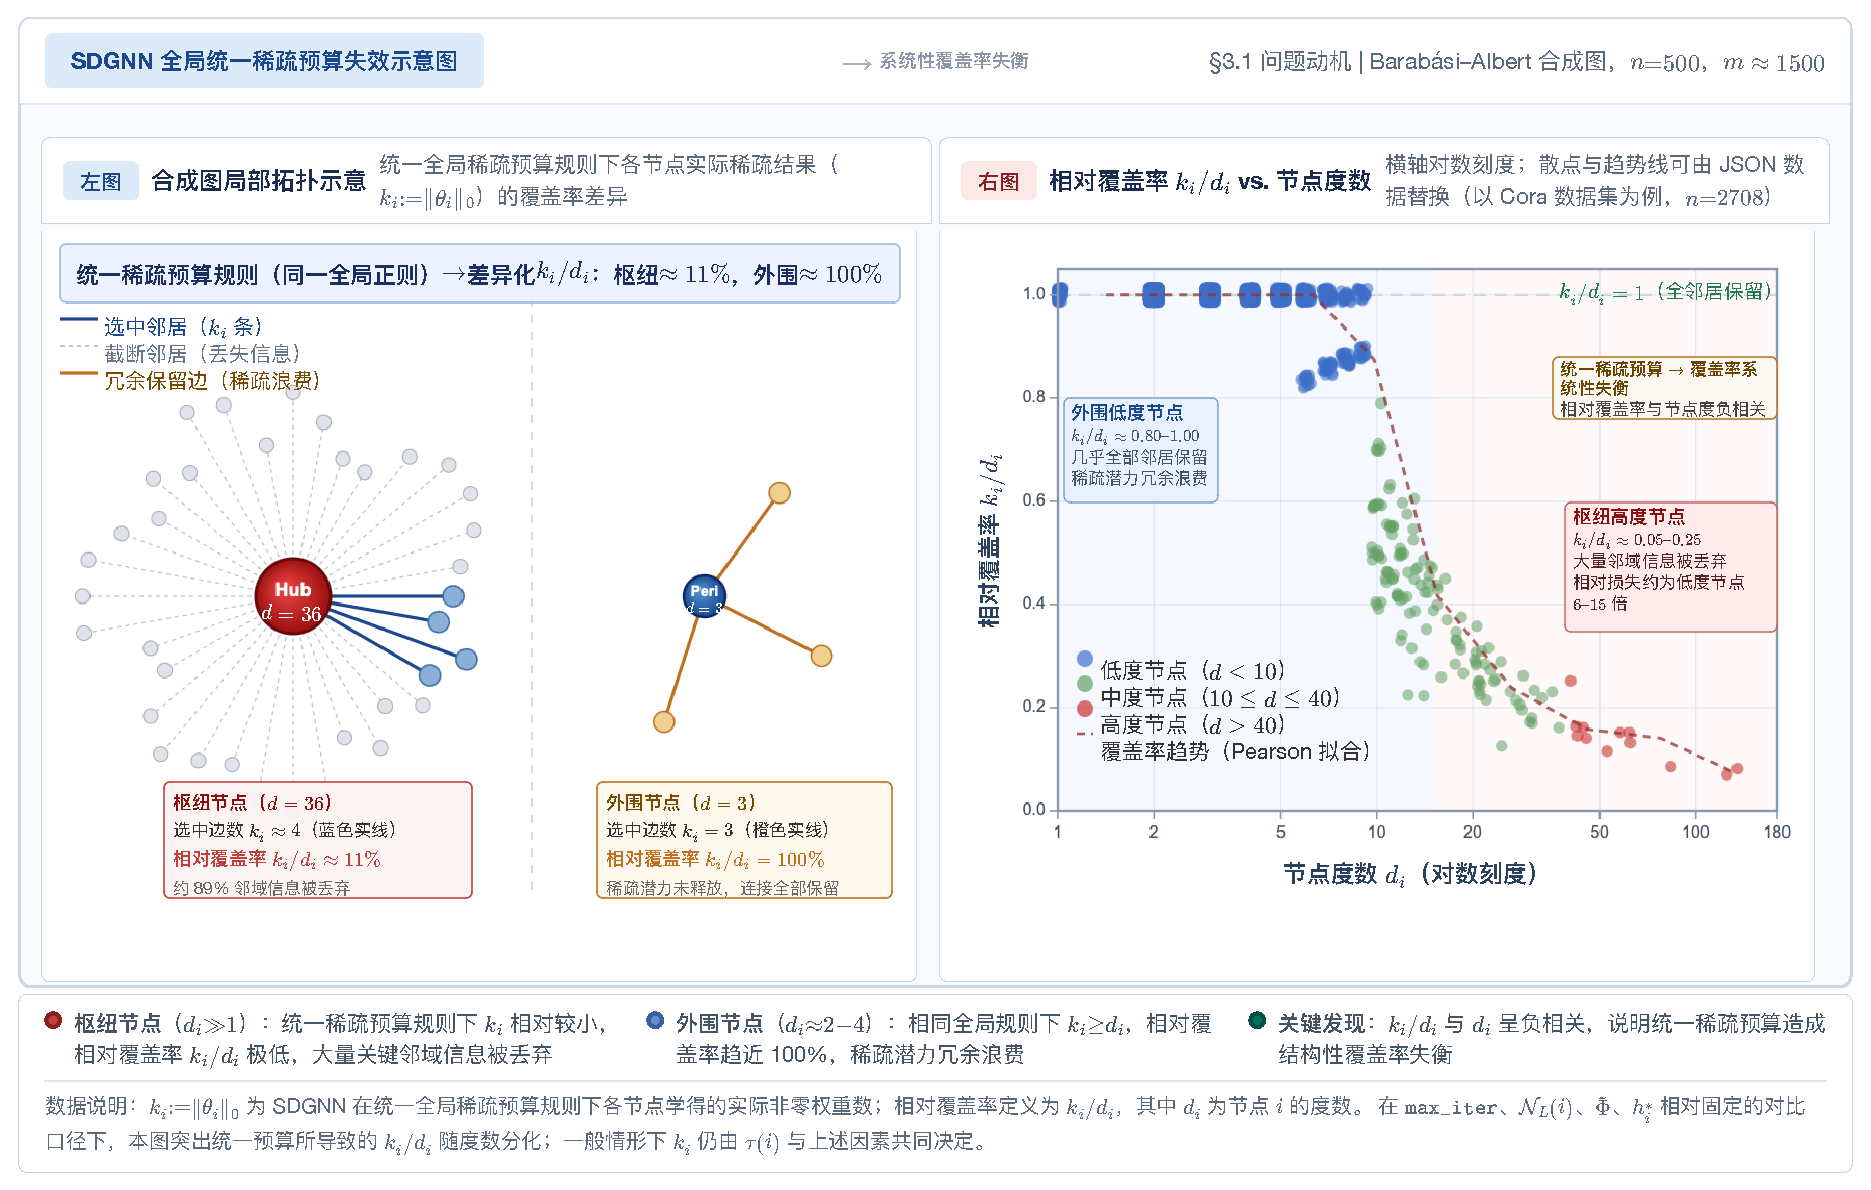
\includegraphics[width=\linewidth]{figures/3-2.pdf}
      \vspace{0.1cm}
      \centering\footnotesize 图3.2：SDGNN全局统一稀疏预算失效示意
    \end{column}
  \end{columns}
\end{frame}

% ==============================================================
% S04  SDGNN 基线与局限
% ==============================================================
\begin{frame}{SDGNN 的突破与局限——本文的问题来源}
  \begin{columns}[T]
    \begin{column}{0.46\textwidth}
      \begin{block}{\green{SDGNN 核心思想}（Hu et al., 2024）}
        \small
        以单次稀疏分解替代多层消息传递，推理阶段仅执行：
        \begin{equation*}
          \hat{H}=\Theta^{\top}\tilde{\Phi}
        \end{equation*}
        $\tilde{\Phi}\in\mathbb{R}^{n\times d}$：预缓存特征；$\Theta\in\mathbb{R}^{n\times n}$：离线固化稀疏权重\\[3pt]
        主项复杂度：$O(L\cdot m\cdot d)\ \longrightarrow$ \highlight{$O(n\kbar d)$}\\[2pt]
        ogbn-arxiv 批次前向：\blue{9.2\,ms}，相对 GCN 加速 $\mathbf{13.6\times}$
      \end{block}

      \vspace{0.2cm}
      \textbf{\highlight{核心局限：全局统一稀疏预算}}
      \begin{itemize}
        \item 以同一 $\lambda_{\mathrm{reg}}$ 约束\textbf{所有节点}
        \item \textbf{枢纽节点}（高度数）：稀疏化过强 $\to$ 丢失关键邻居
        \item \textbf{外围节点}（低度数）：稀疏化不足 $\to$ 保留冗余连接
        \item 复杂图（异配、重尾度）：失配更明显
      \end{itemize}
      \vspace{0.15cm}
      \textbf{本文问题}：能否在保持 $O(n\kbar d)$ 接口不变的前提下，引入\textbf{节点级差异化稀疏预算}？
    \end{column}

    \begin{column}{0.50\textwidth}
      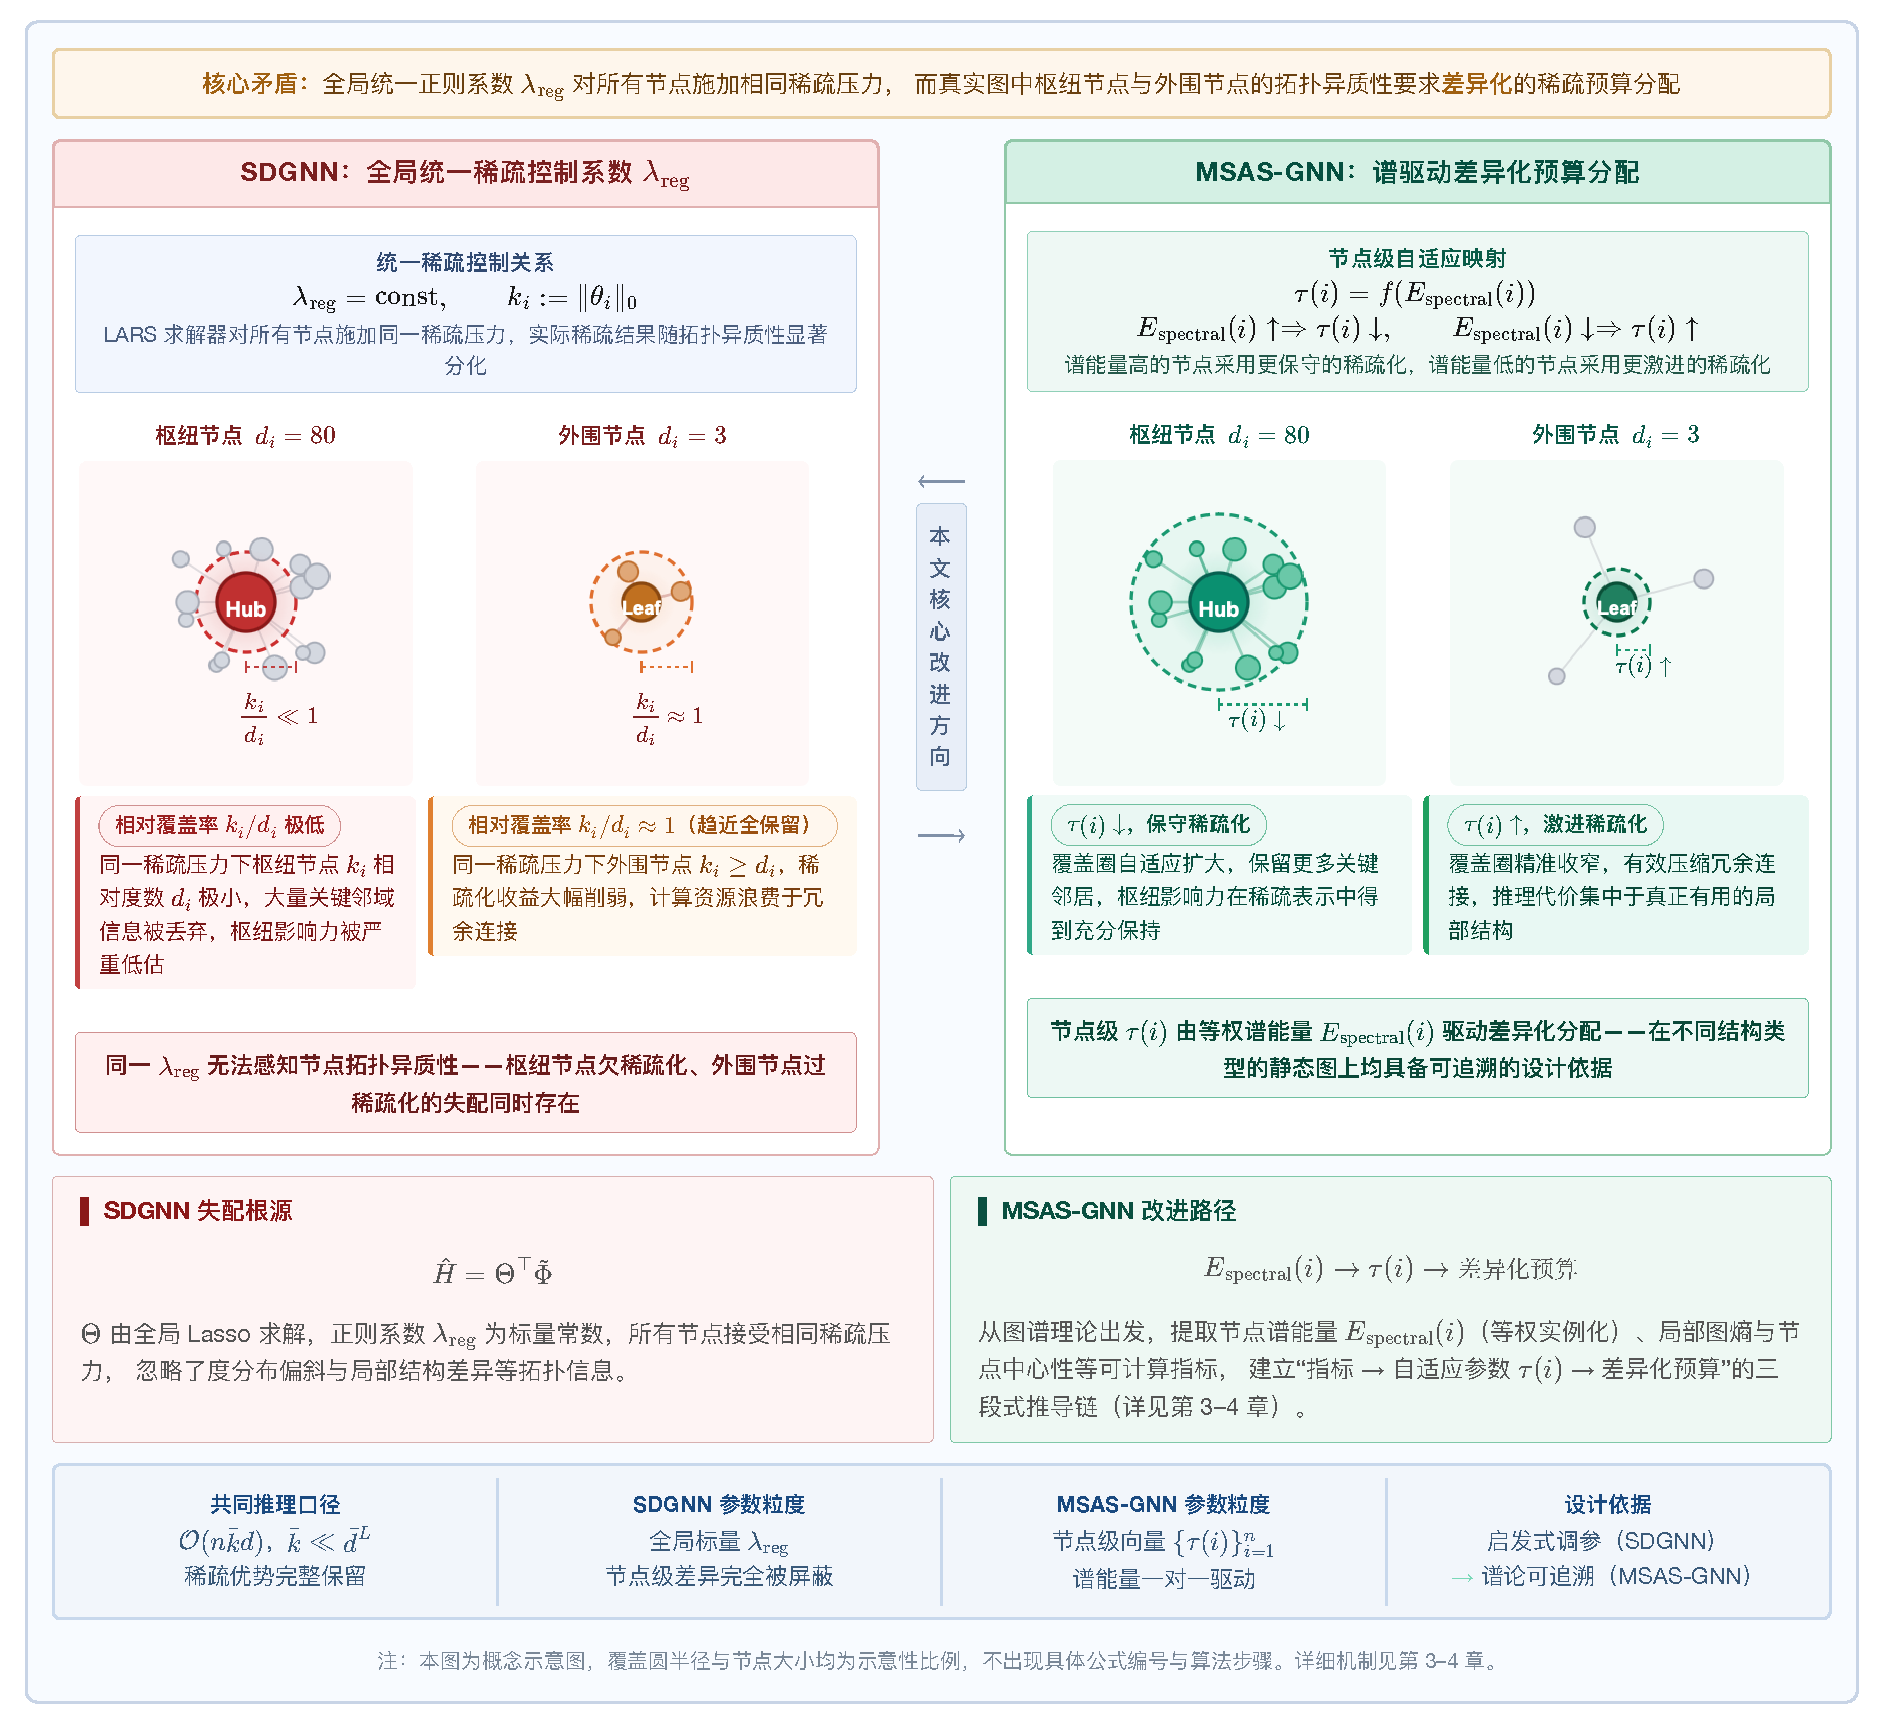
\includegraphics[width=\linewidth]{figures/1-1.pdf}
      \vspace{0.05cm}
      \centering\footnotesize 图1.1：SDGNN全局统一稀疏预算局限与MSAS-GNN自适应改进示意
    \end{column}
  \end{columns}
\end{frame}

% ==============================================================
% S05  研究目标与全文方法链
% ==============================================================
\begin{frame}{研究目标与全文技术路线}
  \begin{columns}[T]
    \begin{column}{0.42\textwidth}
      \textbf{\blue{研究目标}}
      \begin{itemize}
        \item 在保持推理主项复杂度 $O(n\kbar d)$ 不变的前提下
        \item 利用可计算图结构统计量构建节点级差异化稀疏预算
        \item 使不同结构角色的节点获得更匹配的信息保留强度
        \item 设计具有可解释、可分析和可验证依据的参数体系
      \end{itemize}

      \vspace{0.1cm}
      \textbf{\blue{全文方法链（四层递进）}}
      \begin{itemize}
        \item \textbf{第3章}：图复杂度指标提取\\
          $\lambda_{\mathrm{gap}}$、$E_{\mathrm{spectral}}(i)$、$H_{\mathrm{norm}}(i)$、$C_{\mathrm{deg}}(i)$
        \item \textbf{第4章}：三维自适应参数设计\\
          频率维 $w_k(i)$ · 节点维 $\tau(i)$ · 跳距维 $k_i^{(l)}$
        \item \textbf{第5章}：分层LARS算法整合\\
          交替优化 $\to$ 固化 $\Theta^{\mathrm{fixed}}$ $\to$ $O(n\kbar d)$ 推理
        \item \textbf{第6章}：6数据集实验验证\\
          主实验·消融·效率分析
      \end{itemize}
    \end{column}

    \begin{column}{0.55\textwidth}
      \textbf{\blue{各章核心输出接口（方程形式）}}

      \begin{block}{第3章 $\to$ 第4章：图结构统计量}
        \small
        $\lambda_{\mathrm{gap}}=\lambda_2(\tilde{\mathcal{L}}_G)$，\quad
        $E_{\mathrm{spectral}}(i)=\tfrac{1}{K}\sum_{k=1}^{K}\lambda_k|U_{ik}|^2$\\[2pt]
        $H_{\mathrm{norm}}(i)=\log d_i^{-1}\sum_{j\in\mathcal{N}(i)}\log d_i$，\quad
        $C_{\mathrm{deg}}(i)=\tfrac{d_i}{n-1}$，\quad $\mathrm{core}(i)\in\mathbb{Z}^+$
      \end{block}

      \smallskip
      \begin{block}{第4章 $\to$ 第5章：三维自适应参数}
        \small
        \textbf{节点维}：$\tau(i)=\mathrm{clip}\!\left(\dfrac{\tau_{\mathrm{base}}\cdot e^{-\beta_\tau E_{\mathrm{spectral}}(i)/E_{\mathrm{thr}}}}{1+\gamma C_{\mathrm{deg}}+\delta\,\mathrm{core}/k_{\max}+\omega_H H_{\mathrm{norm}}},\,\tau_{\min},\tau_{\mathrm{base}}\right)$\\[4pt]
        \textbf{跳距维}：$k_i^{(l)}=\operatorname{RoundQuota}\!\bigl(\rho\,p_l\,|\mathcal{R}_l(i)|\bigr)\leq|\mathcal{R}_l(i)|$\\[2pt]
        \textbf{频率维}：$w_k(i)=1/K$（等权，任务无关）
      \end{block}

      \smallskip
      \begin{block}{第5章 $\to$ 第6章：推理接口与复杂度}
        \small
        训练输出：$\Theta^{\mathrm{fixed}}\in\mathbb{R}^{n\times n}$（离线固化），$\tilde{\Phi}_{\mathrm{cache}}\in\mathbb{R}^{n\times d}$\\[2pt]
        在线推理：$\hat{H}=(\Theta^{\mathrm{fixed}})^\top\tilde{\Phi}_{\mathrm{cache}}$，
        主项复杂度 \highlight{$O(n\kbar d)$}，$\kbar\ll\bar{d}^L$
      \end{block}
    \end{column}
  \end{columns}
\end{frame}

% ==============================================================
% S06  第3章：问题形式化
% ==============================================================
\section{问题形式化与图复杂度指标}
\setchapternote{第3章}

% ==============================================================
% S06  第3章：问题形式化——SDGNN 的失配与本文优化目标
% ==============================================================

\begin{frame}{问题形式化——为什么需要节点级稀疏预算？}
\begin{columns}[T]

\begin{column}{0.46\textwidth}
  \begin{alertblock}{SDGNN 的系统性失配}
    SDGNN 以同一 $\lambda_{\mathrm{reg}}$ 约束所有节点：
    \begin{equation*}
      \min_{\theta_i}\;\bigl\|h_i^*-\tilde{\Phi}^\top\theta_i\bigr\|_2^2
      +{\color{myred}\lambda_{\mathrm{reg}}}\|\theta_i\|_1,\quad\forall\,i
    \end{equation*}
    真实网络度分布呈长尾甚至幂律分布，方差
    $\mathrm{Var}(\{d_i\})=\frac{1}{n}\sum_i(d_i-\bar{d})^2$ 较大时：

    \medskip
    \begin{tabular}{ll}
      \toprule
      节点类型 & 相同 $\lambda_{\mathrm{reg}}$ 的后果 \\
      \midrule
      高度数节点 & 稀疏化\highlight{过强}，关键邻居被截断 \\
      低度数节点 & 稀疏化\highlight{不足}，冗余连接被保留 \\
      \bottomrule
    \end{tabular}
  \end{alertblock}

  \medskip
  \textbf{\blue{本文目标}}：在保留推理接口 $O(n\kbar d)$ 不变的前提下，引入节点级差异化稀疏约束：
  \begin{equation*}
    \min_{\theta_i}\;\bigl\|h_i^*-\tilde{\Phi}^\top\theta_i\bigr\|_2^2
    +{\color{myred}\tau(i)}\|\theta_i\|_1
    \;\text{s.t.}\;\|\theta_i\|_0\leq\textstyle\sum_l k_i^{(l)}
  \end{equation*}
  $\tau(i)$：节点级正则系数（枢纽节点偏小，外围节点偏大）\\
  $k_i^{(l)}$：第 $l$ 跳环层预算上界（近邻优先）
\end{column}

\begin{column}{0.50\textwidth}
  \textbf{\blue{推理阶段接口不变}}（训练完成后离线固化）：
  \begin{equation*}
    \hat{H}=\bigl(\Theta^{\mathrm{fixed}}\bigr)^\top\tilde{\Phi}_{\mathrm{cache}}
    \quad\Rightarrow\quad O(n\kbar d)
  \end{equation*}

  % \medskip
  \textbf{\blue{三项设计准则}}

  % \medskip
  \begin{tabular}{lm{5cm}}
    \toprule
    准则 & 含义 \\
    \midrule
    \textbf{可解释性} & $\tau(i)$、$k_i^{(l)}$ 由可计算图结构统计量唯一确定，参数意义明确 \\[4pt]
    \textbf{复杂度不变} & 在线推理严格保持 $O(n\kbar d)$，$\kbar\ll\bar{d}^L$ \\[4pt]
    \textbf{任务无关性} & 不依赖标签统计量，等权实例化，避免标签泄漏 \\
    \bottomrule
  \end{tabular}

  % \medskip
  \begin{block}{表示近似误差度量}
    \[
      \mathcal{E}_{\mathrm{approx}}=\frac{1}{\sqrt{n}}\|H^*-\hat{H}\|_F
    \]
    $\mathcal{E}_{\mathrm{approx}}$ 越小 $\Leftrightarrow$ 稀疏支撑集质量越好\\[3pt]
    第5章证明：在 $\sigma$-谱相似性条件下
    $\mathcal{E}_{\mathrm{approx}}\lesssim 2(\sigma-1)C_g\|X\|_F$，\\
    参数设计方向：令 $\sigma\to 1$
  \end{block}
\end{column}
\end{columns}
\end{frame}

% ==============================================================
% S07  第3章：四类图复杂度指标——τ(i) 和 k_i^(l) 的原材料
% ==============================================================
\begin{frame}{四类图复杂度指标——$\tau(i)$ 与 $k_i^{(l)}$ 的输入原材料}
\begin{columns}[T]

\begin{column}{0.50\textwidth}
  \textbf{\blue{（1）谱间隙 $\lambda_{\mathrm{gap}}$}}（全图级 · 频率维 / 跳距维）

  归一化拉普拉斯 $\tilde{\mathcal{L}}=U\Lambda U^\top$ 的最小非零特征值：
  \begin{equation*}
    \lambda_{\mathrm{gap}}:=\lambda_1,\qquad
    0=\lambda_0<\lambda_1\leq\cdots\leq\lambda_{n-1}\leq 2
  \end{equation*}
  刻画图的代数连通强度；$\lambda_{\mathrm{gap}}$ 大 $\Rightarrow$ 近跳信息充足 $\Rightarrow$ 远跳可更强稀疏化\\
  \textbf{接口}：驱动第4章§\,4.3.2 分层跳距保留率策略

  \vspace{1cm}
  \textbf{\blue{（2）节点谱能量 $E_{\mathrm{spectral}}(i)$}}（节点级 · 频率维）
  \begin{equation*}
    E_{\mathrm{spectral}}(i)=\sum_{k=1}^{K_{\mathrm{pair}}} w_k\,|U_{ik}|^2,\quad
    w_k=\tfrac{1}{K_{\mathrm{pair}}}\ (\text{等权，任务无关})
  \end{equation*}
  节点 $i$ 在非平凡谱分量上的参与强度；\\
  $E_{\mathrm{spectral}}(i)\uparrow\Rightarrow$ 高频参与强 $\Rightarrow\tau(i)\downarrow$（保留更多邻居）\\
  \textbf{接口}：$\tau(i)$ 多因子融合的\textbf{核心谱输入}
\end{column}

\begin{column}{0.46\textwidth}
  \textbf{\blue{（3）归一化局部图熵 $H_{\mathrm{norm}}(i)$}}（节点级 · 节点维）

  基于 Gaussian 核边权 $w_{ij}\propto\exp(-\|x_i-x_j\|^2/2\sigma^2)$：
  \begin{equation*}
    H_{\mathrm{norm}}(i)=
    -\frac{\sum_{j\in\mathcal{N}(i)}\hat{w}_{ij}\ln\hat{w}_{ij}}
          {\ln|\mathcal{N}(i)|},\quad
    \hat{w}_{ij}=\frac{w_{ij}}{\sum_{k}w_{ik}}
  \end{equation*}
  刻画邻域消息流的均匀/分散程度（含特征相似性信息）；\\
  $H_{\mathrm{norm}}\uparrow\Rightarrow$ 邻域多样 $\Rightarrow\tau(i)\downarrow$\\
  \textbf{接口}：进入 $\tau(i)$ 多因子融合（第4章§\,4.2.2）

  \medskip
  \textbf{\blue{（4）度中心性 $C_{\mathrm{deg}}(i)$ 与 $k$-core 指数}}（节点维）
  \begin{equation*}
    C_{\mathrm{deg}}(i)=\frac{d_i}{n-1},\qquad
    \mathrm{core}(i)=\max\{k: i\in G_k\}
  \end{equation*}
  $G_k$：子图内任意节点度 $\geq k$ 的极大诱导子图（$k$-core）；\\
  枢纽节点（$C_{\mathrm{deg}}\uparrow,\mathrm{core}\uparrow$）$\Rightarrow\tau(i)\downarrow$\\
  \textbf{接口}：进入 $\tau(i)$ 多因子融合（第4章§\,4.2.2）

  % \medskip
  % \begin{alertblock}{四类指标汇总接口}
  %   \small
  %   \begin{tabular}{p{2.2cm}p{1.8cm}p{1.4cm}}
  %     指标 & 维度归属 & 接入第4章 \\
  %     \midrule
  %     $\lambda_{\mathrm{gap}}$ & 全图·跳距 & §\,4.3.2 \\
  %     $E_{\mathrm{spectral}}(i)$ & 节点·频率 & §\,4.2.2 + §\,4.1 \\
  %     $H_{\mathrm{norm}}(i)$ & 节点·节点维 & §\,4.2.2 \\
  %     $C_{\mathrm{deg}}(i),\mathrm{core}(i)$ & 节点·节点维 & §\,4.2.2 \\
  %   \end{tabular}
  % \end{alertblock}
\end{column}
\end{columns}
\end{frame}

% ==============================================================
% S07b  第3章：算法3.1——四类指标如何统一计算？
% ==============================================================
\begin{frame}{算法3.1——四类指标的离线统一预处理}
\begin{columns}[T]

\begin{column}{0.6\textwidth}
  \textbf{\blue{算法3.1：图复杂度指标预处理}}

  \vspace{-2.7pt}
  \small
  \begin{algorithmic}[1]
    \Require $G=(V,E,X)$；$\tilde{\mathcal{L}}$；$K_{\mathrm{eig}}$
    \Ensure $\hat{\lambda}_{\mathrm{gap}}$；$\{(\lambda_k,u_k)\}$；$\{E_{\mathrm{spectral}}(i)\}$；$\{H_{\mathrm{norm}}(i)\}$；$\{C_{\mathrm{deg}}(i)\}$；$\{\mathrm{core}(i)\}$
    \State \textit{第一阶段：Lanczos 截断谱估计，$O(mK_{\mathrm{eig}})$}
    \State Lanczos 迭代得 $\hat{\lambda}_{\mathrm{gap}}$，$K_{\mathrm{pair}}\leftarrow\min(K_{\mathrm{eig}},K_{\mathrm{eff}}{-}1)$，$\{(\lambda_r,u_r)\}_{r=1}^{K_{\mathrm{pair}}}$
    \State \textit{第二阶段：节点谱能量批量计算（等权实例化），$O(nK_{\mathrm{eig}})$}
    \State $U\leftarrow[u_1,\ldots,u_{K_{\mathrm{pair}}}]$
    \For{$i=1$ \textbf{to} $n$}
      \State $E_{\mathrm{spectral}}(i)\leftarrow\dfrac{1}{K_{\mathrm{pair}}}\displaystyle\sum_{k=1}^{K_{\mathrm{pair}}}\lambda_k\,|U_{ik}|^2$
    \EndFor
    \State \textit{第三阶段：Gaussian 图熵、度中心性与 $k$-core，$O(mD){+}O(m)$}
    \State $\hat{\sigma}^2\leftarrow\mathrm{median}(\{\|x_i-x_j\|^2:(i,j)\in E\})$；$\gamma_x\leftarrow1/(2\hat{\sigma}^2)$
    \State $\forall(i,j)\in E$：$w_{ij}\leftarrow\exp(-\gamma_x\|x_i-x_j\|^2)$
    \For{$i=1$ \textbf{to} $n$}
      \State $Z_i\leftarrow\sum_{j\in\mathcal{N}(i)}w_{ij}$
      \If{$|\mathcal{N}(i)|>1$}\enspace $H_{\mathrm{norm}}(i)\leftarrow{-}\tfrac{1}{\ln|\mathcal{N}(i)|}\sum_{j}\tfrac{w_{ij}}{Z_i}\ln\tfrac{w_{ij}}{Z_i}$
      \Else\enspace $H_{\mathrm{norm}}(i)\leftarrow 0$
      \EndIf
      \State $C_{\mathrm{deg}}(i)\leftarrow d_i/(n-1)$
    \EndFor
    \State Batagelj--Zaversnik 剥核算法：$\{\mathrm{core}(i)\}_{i=1}^n$，$O(m)$
  \end{algorithmic}
\end{column}

\begin{column}{0.4\textwidth}
  \textbf{\blue{三阶段流水线示意}}

  \medskip
  \begin{tikzpicture}[
      node distance=0.32cm,
      box/.style={rounded corners=3pt, draw=mynavy, fill=mynavy!8,
                  text width=4.6cm, align=left, font=\small,
                  inner sep=4pt},
      mainbox/.style={rounded corners=3pt, draw=myred, fill=myred!8,
                  text width=4.6cm, align=left, font=\small,
                  inner sep=4pt},
      outbox/.style={rounded corners=3pt, draw=mygreen, fill=mygreen!8,
                  text width=4.6cm, align=left, font=\small,
                  inner sep=4pt},
      arr/.style={->, thick, color=gray!70}
    ]
    \node[box] (in) {\textbf{输入}：$G=(V,E,X)$，$\tilde{\mathcal{L}}$，$K_{\mathrm{eig}}$};
    \node[box, below=of in] (s1)
      {\textbf{阶段一}（简写）\\
       Lanczos 截断谱估计\\
       $\Rightarrow\hat{\lambda}_{\mathrm{gap}},\;\{(\lambda_k,u_k)\}_{k=1}^{K_{\mathrm{pair}}}$\\
       \textcolor{gray}{复杂度 $O(mK_{\mathrm{eig}})$}};
    \node[mainbox, below=of s1] (s2)
      {\textbf{阶段二（主线）}\\
       $\forall i$：$E_{\mathrm{spectral}}(i)\leftarrow\frac{1}{K_{\mathrm{pair}}}\sum_k\lambda_k|U_{ik}|^2$\\
       等权实例化，任务无关\\
       \textcolor{gray}{复杂度 $O(nK_{\mathrm{eig}})$}};
    \node[box, below=of s2] (s3)
      {\textbf{阶段三}（简写）\\
       $H_{\mathrm{norm}}(i)$（Gaussian 核）；$C_{\mathrm{deg}}(i)$；\\
       $\mathrm{core}(i)$（剥核，$O(m)$）\\
       \textcolor{gray}{复杂度 $O(mD)+O(m)$}};
    \node[outbox, below=of s3] (out)
      {\textbf{缓存输出} $\to$ 第4章参数化};
    \draw[arr] (in) -- (s1);
    \draw[arr] (s1) -- (s2);
    \draw[arr] (s2) -- (s3);
    \draw[arr] (s3) -- (out);
  \end{tikzpicture}

  % \medskip
  % \begin{alertblock}{与后续章节的接口}
  %   \begin{tabular}{p{2.0cm}p{3.0cm}}
  %     $\hat{\lambda}_{\mathrm{gap}}$ & $\to$ 第4章§\,4.3.2\\
  %     & 分层跳距保留率 \\[3pt]
  %     $E_{\mathrm{spectral}}(i)$ & $\to$ 第4章§\,4.2.2\\
  %     & $\tau(i)$ 谱输入因子 \\[3pt]
  %     $H_{\mathrm{norm}},C_{\mathrm{deg}},\mathrm{core}$ & $\to$ 第4章§\,4.2.2\\
  %     & $\tau(i)$ 结构因子 \\
  %   \end{tabular}
  % \end{alertblock}
\end{column}
\end{columns}
\end{frame}

% ==============================================================
% S08  第4章：三维自适应稀疏机制——整体框架
% ==============================================================
\section{三维自适应稀疏机制}
\setchapternote{第4章}

\begin{frame}{三维自适应稀疏机制——放松三条隐含假设}
\begin{columns}[T]

\begin{column}{0.32\textwidth}
  \begin{block}{\blue{频率维（§\,4.1）}}
    \small
    \textbf{放松假设}：统一低通传播\\[4pt]
    \textbf{核心公式}：
    \begin{equation*}
      E_{\mathrm{spectral}}(i)
      =\frac{1}{K}\sum_{k=1}^{K}\lambda_k|U_{ik}|^2
    \end{equation*}
    谱输入权重 $w_k(i)=1/K$（等权）\\[4pt]
    \textbf{设计选择}：等权而非同配率加权\\
    $\Rightarrow$ 任务无关，不绑定标签\\
    $\Rightarrow$ 作为节点维的谱强度输入
  \end{block}
\end{column}

\begin{column}{0.34\textwidth}
  \begin{alertblock}{\highlight{节点维（§\,4.2）}}
    \small
    \textbf{放松假设}：统一稀疏压力\\[4pt]
    \textbf{三步构造}：\\
    (1) 单调原则：$E\uparrow\Rightarrow\tau(i)\downarrow$\\
    (2) 单因子基线：$\tau_{\mathrm{mono}}(i)=\mathrm{clip}(\tau_{\mathrm{base}} e^{-\beta_\tau E/E_{\mathrm{thr}}},\tau_{\min},\tau_{\mathrm{base}})$\\[2pt]
    (3) 多因子完整式：
    {\tiny
    \begin{equation*}
      \hspace{-0.6cm}\tau(i)=\mathrm{clip}\!\left(
      \frac{\tau_{\mathrm{base}} e^{-\beta_\tau E_i/E_{\mathrm{thr}}}}
           {1+\gamma C_{\mathrm{deg}}+\delta\frac{\mathrm{core}}{k_{\max}}+\omega_H H_{\mathrm{norm}}},
      \tau_{\min},\tau_{\mathrm{base}}\!\right)
    \end{equation*}
    }
    参数默认值：$(\beta_\tau,\gamma,\delta,\omega_H)=(1.0,0.5,0.3,0.2)$
  \end{alertblock}
\end{column}

\begin{column}{0.32\textwidth}
  \begin{exampleblock}{\green{跳距维（§\,4.3）}}
    \small
    \textbf{放松假设}：各跳贡献均等\\[4pt]
    \textbf{衰减界}（§\,4.3.1）：
    \begin{equation*}
      \|\Delta h_i^{[l]}\|_2\le C_0\,\mu_\star(P)^{l-1}
    \end{equation*}
    边际贡献按几何速度衰减\\[4pt]
    \textbf{保留率策略}（策略1）：
    \begin{equation*}
      p_l=p_1\cdot\varrho^{l-1},\;\varrho\in(0,1)
    \end{equation*}
    \textbf{分层预算配额}：
    \begin{equation*}
      k_i^{(l)}=\operatorname{RoundQuota}(\rho\,p_l\,|\mathcal{R}_l(i)|)
    \end{equation*}
  \end{exampleblock}
\end{column}

\end{columns}

\vspace{0.05cm}
\centering
\begin{tabular}{m{1.4cm}m{3cm}m{1.8cm}m{2.8cm}m{2cm}}
  \toprule
  \textbf{维度} & \textbf{放松的假设} & \textbf{参数} & \textbf{驱动统计量} & \textbf{接口} \\
  \midrule
  频率维 & 统一低通传播适合所有节点 & $w_k(i)=1/K$ & $E_{\mathrm{spectral}}(i)$ & $\tau(i)$ 谱输入 \\
  节点维 & 节点适合相同稀疏压力 & $\tau(i)$ & $E,H_{\mathrm{norm}},C_{\mathrm{deg}},\mathrm{core}$ & Phase\,$\Theta$ 正则 \\
  跳距维 & 各跳距邻居贡献均等 & $k_i^{(l)}$ & $\lambda_{\mathrm{gap}},|\mathcal{R}_l(i)|$ & Phase\,$\Theta$ 截断 \\
  \bottomrule
\end{tabular}
\end{frame}
% ==============================================================
% S09  τ(i)：不同节点的稀疏约束为何不同，如何计算？
% ==============================================================
\begin{frame}{节点维 $\tau(i)$：哪类节点应保留更多邻居？（§\,4.2）}
\begin{columns}[T]

\begin{column}{0.48\textwidth}
  \begin{alertblock}{核心问题}
    SDGNN 对所有节点施加同一正则强度 $\lambda_{\mathrm{reg}}$——\\
    枢纽节点（高度数、高$k$-core）稀疏化\textbf{过强}，\\
    外围节点稀疏化\textbf{不足}。\\[3pt]
    \textbf{本节目标}：为每个节点设计差异化的正则系数 $\tau(i)$
  \end{alertblock}

  \vspace{0.15cm}
  \textbf{\blue{单调性设计原则}}

  结构信息贡献越大的节点 $\Rightarrow$ $\ell_1$ 惩罚越弱 $\Rightarrow$ 保留邻居越多：
  \begin{equation*}
    E_{\mathrm{spectral}}(i)\uparrow,\;
    C_{\mathrm{deg}}(i)\uparrow,\;
    \mathrm{core}(i)\uparrow,\;
    H_{\mathrm{norm}}(i)\uparrow
    \;\Rightarrow\;\tau(i)\downarrow
  \end{equation*}

  \vspace{0.1cm}
  \textbf{\blue{多因子融合公式}}（§\,4.2.2）
     {\small
     \begin{equation*}
      \tau(i)=\mathrm{clip}\!\!\left(
      \frac{\tau_{\mathrm{base}}\cdot
      \exp\!\bigl(-\beta_\tau E_{\mathrm{spectral}}(i)/E_{\mathrm{thr}}\bigr)}
      {1+\gamma C_{\mathrm{deg}}+\delta\,\mathrm{core}/k_{\max}+\omega_H H_{\mathrm{norm}}},\;
      \tau_{\min},\,\tau_{\mathrm{base}}\right)
    \end{equation*}
    $\gamma=\delta=\omega_H=0$ 时退化为仅谱能量的单因子基线；\\
    分母 $>1$，各结构因子贡献方向一致，$\partial\tau/\partial\alpha_i<0$ 严格成立
     }

  % \begin{block}{}
  %   \small
  %   \[
  %     \tau(i)=\mathrm{clip}\!\!\left(
  %     \frac{\tau_{\mathrm{base}}\cdot
  %     \exp\!\bigl(-\beta_\tau E_{\mathrm{spectral}}(i)/E_{\mathrm{thr}}\bigr)}
  %     {1+\gamma C_{\mathrm{deg}}+\delta\,\mathrm{core}/k_{\max}+\omega_H H_{\mathrm{norm}}},\;
  %     \tau_{\min},\,\tau_{\mathrm{base}}\right)
  %   \]
  %   $\gamma=\delta=\omega_H=0$ 时退化为仅谱能量的单因子基线；\\
  %   分母 $>1$，各结构因子贡献方向一致，$\partial\tau/\partial\alpha_i<0$ 严格成立
  % \end{block}
\end{column}

\begin{column}{0.48\textwidth}
  \textbf{\blue{不同节点类型的 $\tau(i)$ 对比}}

  \vspace{0.05cm}
  \small
  \begin{tabular}{llll}
    \toprule
    节点类型 & $\tau(i)$ & 保留邻居 & 直觉 \\
    \midrule
    枢纽\\（高度、高core） & \green{偏小} & 较多 & 跨区信息传递关键 \\[4pt]
    外围\\（低度、低core） & \highlight{偏大} & 较少 & 局部冗余多 \\[4pt]
    普通节点 & 中等 & 中等 & 均衡处理 \\
    \bottomrule
  \end{tabular}

  \vspace{0.2cm}
  \textbf{\blue{默认参数与稳健区间}}

  \vspace{0.05cm}
  \small
  \begin{tabular}{llll}
    \toprule
    参数 & 默认值 & 稳健区间 & 控制对象 \\
    \midrule
    $\beta_\tau$ & 1.0 & [0.8, 1.2] & 谱能量响应 \\
    $\gamma$ & 0.5 & [0.3, 0.8] & 度中心性权重 \\
    $\delta$ & 0.3 & [0.2, 0.5] & $k$-core 权重 \\
    $\omega_H$ & 0.2 & [0.1, 0.4] & 局部图熵权重 \\
    $\tau_{\mathrm{base}}$ & $10^{-3}$ & $[10^{-4}, 10^{-2}]$ & 正则基准值 \\
    \bottomrule
  \end{tabular}

    % \begin{tabular}{ll}
    %   SDGNN（统一 $\lambda$） & 无差异化 \\
    %   仅谱能量 & $E\uparrow\Rightarrow\tau\downarrow$ \\
    %   $+$ 度中心性 & $C_{\mathrm{deg}}\uparrow\Rightarrow\tau\downarrow$ \\
    %   \textbf{+ core + 图熵（本文）} & \textbf{结构越重要$\Rightarrow\tau$越小} \\
    % \end{tabular}

  % \vspace{0.15cm}
  \begin{block}{因子渐进方案（§\,4.2.1，详见§\,6.3消融）}
    \small
    \begin{tabular}{ll}
      SDGNN（统一 $\lambda$） & 无差异化 \\
      仅谱能量 & $E\uparrow\Rightarrow\tau\downarrow$ \\
      $+$ 度中心性 & $C_{\mathrm{deg}}\uparrow\Rightarrow\tau\downarrow$ \\
      \textbf{+ core + 图熵（本文）} & \textbf{结构越重要$\Rightarrow\tau$越小} \\
    \end{tabular}
  \end{block}
\end{column}
\end{columns}
\end{frame}

% ==============================================================
% S10a  跳距衰减界：近跳比远跳重要，有数学证明
% ==============================================================
\begin{frame}{跳距维（一）：近跳贡献更大——信息衰减界（§\,4.3.1）}
\begin{columns}[T]

\begin{column}{0.50\textwidth}
  \begin{alertblock}{核心问题}
    \small 各跳邻居对节点表示的贡献相同吗？\\
    \textbf{结论}：不同——近跳贡献有数学上界，随跳距几何衰减
  \end{alertblock}

  \vspace{0.05cm}
  {\small
  \textbf{\blue{三步推导：第 $l$ 跳边际贡献的上界}}

  设 $P$ 为归一化传播算子，$\mu_\star(P)$ 为第二谱半径：

  \textbf{(1) 标准基展开}
  \begin{equation*}
    \|\Delta h_i^{[l]}\|_2 \le \|P^{l-1}(P-I)X\|_F
  \end{equation*}

  \textbf{(2) 非主方向几何收缩}（主特征方向被 $(P-I)$ 抵消）
  \begin{equation*}
    \|P^{l-1}(P-I)X\|_F \le \mu_\star(P)^{l-1} \cdot \underbrace{\|(P-I)X\|_F}_{C_0}
  \end{equation*}

  \vspace{-0.3cm}

  \textbf{(3) 核心衰减界}（合并得到）
  \begin{equation*}
    \boxed{\|\Delta h_i^{[l]}\|_2 \;\le\; C_0\,\mu_\star(P)^{l-1}}
  \end{equation*}
  $\mu_\star(P)<1$ 时，边际贡献上界随 $l$ 增大\textbf{按几何速度衰减}。

  \vspace{0.1cm}
  \textbf{(4) 保留率参考下界}：令未保留损失 $(1-p_l)C_0\mu_\star^{l-1}\le\varepsilon_l$，得
  \begin{equation*}
    p_l \;\geq\; \max\!\left\{0,\;1 - \frac{\varepsilon_l}{C_0\,\mu_\star(P)^{l-1}}\right\}
  \end{equation*}
  \highlight{$l$ 增大 $\Rightarrow$ 下界降低 $\Rightarrow$ 远跳可以更强稀疏化}
  }
\end{column}

\begin{column}{0.46\textwidth}
  \textbf{\blue{谱间隙如何影响衰减速度}}（§\,4.3.2）

  由 $\tilde{\mathcal{L}}=I-S$ 推出 $\lambda_k=1-\mu_k(S)$，对低频非平凡方向：
  \begin{equation*}
    \mu_2(S)=1-\lambda_{\mathrm{gap}}
  \end{equation*}

  \vspace{0.03cm}
  
  \begin{tabular}{lll}
    \toprule
    $\lambda_{\mathrm{gap}}$ & $\mu_2(S)$ & 衰减速度 \\
    \midrule
    大（连通性强） & 小 & 快 $\Rightarrow$ 远跳更可稀疏 \\
    小（图稀疏） & 接近 1 & 慢 $\Rightarrow$ 远跳仍需保留 \\
    \bottomrule
  \end{tabular}

  \vspace{0.05cm}
  \begin{alertblock}{口径说明}
     $\mu_2(S)=1-\lambda_{\mathrm{gap}}$ 只刻画低频非平凡方向，不等同于 $\mu_\star(S)$。本文以 $\hat{\lambda}_{\mathrm{gap}}$ 作为代理量
  \end{alertblock}

  \vspace{0.08cm}
  \textbf{\blue{结论：分层预算应"近多远少"}}

  \vspace{0.03cm}
  \begin{tabular}{lll}
    \toprule
    跳距 $l$ & 衰减因子上界 & 建议保留率 \\
    \midrule
    1（近邻） & $C_0$ & 最高 $p_1$ \\
    2 & $C_0\mu_\star$ & 次之 $p_2 < p_1$ \\
    3 & $C_0\mu_\star^2$ & 更低 $p_3 < p_2$ \\
    $L$（远端） & $C_0\mu_\star^{L-1}$ & 最低 $p_L$ \\
    \bottomrule
  \end{tabular}

  \vspace{0.05cm}
  \footnotesize 这是策略设计的理论动机；下页给出两种具体策略
\end{column}
\end{columns}
\end{frame}

% ==============================================================
% S10b  跳距维（二）：p_l 如何设计，k_i^(l) 如何计算？
% ==============================================================
\begin{frame}{跳距维（二）：$p_l$ 两种策略与整数预算分配公式（§\,4.3.2--4.3.3）}
\begin{columns}[T]

\begin{column}{0.50\textwidth}
  \textbf{\blue{策略1：均匀衰减（首末比率可控）}}
  \begin{equation*}
    p_l = p_1\cdot\varrho^{l-1},\qquad
    \varrho=\!\left(\frac{p_L}{p_1}\right)^{\!\frac{1}{L-1}}\!\in(0,1)
  \end{equation*}
  给定首末跳保留率 $p_1$、$p_L$，中间各跳自动确定。

  \textit{示例}：$L=3,\;p_1=0.60,\;p_3=0.20$\\
  $\Rightarrow\;(p_1,p_2,p_3)=(0.60,\;0.40,\;0.20)$

  \vspace{0.1cm}
  \textbf{\blue{策略2：谱间隙自适应（衰减速度图适应）}}

  以预处理阶段得到的 $\hat{\lambda}_{\mathrm{gap}}$ 为代理量：
  \begin{equation*}
    r=\exp(-\kappa\hat{\lambda}_{\mathrm{gap}})\in(0,1],\qquad
    p_l=\max\!\bigl\{p_{\min},\;p_1\cdot r^{l-1}\bigr\}
  \end{equation*}
  $\hat{\lambda}_{\mathrm{gap}}$ 大 $\Rightarrow$ $r$ 小 $\Rightarrow$ 远跳衰减快；$p_{\min}=0.1$ 防止完全压缩

  \vspace{0.08cm}
  \small
  \begin{tabular}{lll}
    \toprule
    & 策略1（均匀） & 策略2（谱间隙自适应） \\
    \midrule
    公比 & 固定 $\varrho$ & 图适应 $r(\hat{\lambda}_{\mathrm{gap}})$ \\
    参数 & $p_1,\;p_L$ & $p_1,\;\kappa,\;p_{\min}$ \\
    理论依据 & 几何递减规律 & $\hat{\lambda}_{\mathrm{gap}}$ 代理低频收缩速度 \\
    \bottomrule
  \end{tabular}
\end{column}

\begin{column}{0.46\textwidth}
  \textbf{\blue{整数预算分配——联合容量约束}}（§\,4.3.3）

  仅有保留率 $p_l$ 不够——还需结合各跳环层的实际邻居容量 $|\mathcal{R}_l(i)|$：
  \begin{equation*}
      k_i^{(l)}
      =\operatorname{RoundQuota}\!\bigl(\rho\,p_l\,|\mathcal{R}_l(i)|\bigr)
      \;\leq\;|\mathcal{R}_l(i)|
    \end{equation*}
      $\rho\in(0,1]$：全局压缩系数；$\operatorname{RoundQuota}$：先下取整再补最大小数部分，保证整数总量等于目标值。
  
  % \begin{block}{}
  %   \begin{equation*}
  %     k_i^{(l)}
  %     =\operatorname{RoundQuota}\!\bigl(\rho\,p_l\,|\mathcal{R}_l(i)|\bigr)
  %     \;\leq\;|\mathcal{R}_l(i)|
  %   \end{equation*}
  %   \small $\rho\in(0,1]$：全局压缩系数；$\operatorname{RoundQuota}$：先下取整再补最大小数部分，保证整数总量等于目标值。
  % \end{block}

  % \vspace{0.1cm}
  \textbf{\blue{节点维 $\tau(i)$ 与跳距维 $k_i^{(l)}$ 的分工}}

  % \vspace{0.05cm}
  \begin{tabular}{m{1cm}m{1cm}m{3.5cm}}
    \toprule
    维度 & 参数 & 回答的问题 \\
    \midrule
    节点维 & $\tau(i)$ & 节点 $i$ 整体应承受\textbf{多强}的稀疏约束？ \\[4pt]
    跳距维 & $k_i^{(l)}$ & 第 $l$ 跳环层最多允许保留\textbf{多少}个邻居？ \\
    \bottomrule
  \end{tabular}

  \vspace{-0.08cm}
  \begin{alertblock}{重要口径}
     $k_i^{(l)}$ 是\textbf{上界}，非固定非零数——实际非零数还由 $\tau(i)$ 的 Lasso 正则强度、LARS 路径提前停止及候选集容量共同决定。$\tau(i)$ 与 $k_i^{(l)}$ 在第5章分层 LARS 的 Phase\,$\Theta$ 中\textbf{联合发挥作用}
  \end{alertblock}
\end{column}
\end{columns}
\end{frame}

% ==============================================================
% S10c-1  两种 LARS 方案：为什么选残差级联？
% ==============================================================
\section{算法整合与理论分析}
\setchapternote{第5章}

\begin{frame}{算法整合：为什么选残差级联 LARS 而非共享目标？（§\,5.1）}
\begin{columns}[T]

\begin{column}{0.47\textwidth}
  \begin{block}{\textbf{\highlight{方案1：共享目标（未采用）}}}
      各层均以同一目标 $\Omega_i=H_{i,:}^*$ 为拟合对象：
    \begin{equation*}
      \theta_{i}^{(l)}
      =\operatorname*{argmin}_\theta
      \bigl\|\tilde{\Phi}_{\mathcal{R}_l}^\top\theta-\Omega_i\bigr\|_2^2
      +\tau(i)\|\theta\|_1,\quad l=0,\ldots,L
    \end{equation*}
    \textbf{问题}：
    \begin{itemize}\setlength{\itemsep}{1pt}
      \item 各层\textbf{独立}逼近同一目标 $\Rightarrow$ 跨层重复，引入冗余
      \item 近跳已解释主要分量后，远跳继续对 $\Omega_i$ 独立拟合，与"近跳优先"预算动机\textbf{相悖}
    \end{itemize}
  \end{block}
\end{column}

\begin{column}{0.49\textwidth}
  \begin{alertblock}{\textbf{\green{方案2：残差级联（本文采用）}}}
      先处理自特征通道，再对\textbf{剩余误差}逐层补偿：\\[3pt]
    \textbf{第0步}（自节点）：
    \begin{equation*}
      \theta_i^{(0)}=\operatorname*{argmin}_\alpha
      \|\alpha\tilde{\phi}_i-\Omega_i\|_2^2+\tau(i)|\alpha|,\quad
      r_i^{(0)}=\Omega_i-\theta_i^{(0)}\tilde{\phi}_i
    \end{equation*}
    \textbf{第 $l$ 步}（$l=1,\ldots,L$，截断上界 $k_i^{(l)}$）：
    \begin{equation*}
      \theta_i^{(l)}=\operatorname*{argmin}_\theta
      \|\tilde{\Phi}_{\mathcal{R}_l}^\top\theta-r_i^{(l-1)}\|_2^2
      +\tau(i)\|\theta\|_1
    \end{equation*}
    \begin{equation*}
      r_i^{(l)}:=r_i^{(l-1)}-\tilde{\Phi}_{\mathcal{R}_l}^\top\theta_i^{(l)}
    \end{equation*}
  \end{alertblock}
\end{column}

\end{columns}

\vspace{0.08cm}
% \small
\begin{tabular}{p{2.2cm}p{5.3cm}p{5.3cm}}
  \toprule
  & \textbf{方案1（共享目标）} & \textbf{方案2（残差级联，本文）} \\
  \midrule
  各层拟合对象 & 均为 $\Omega_i$，层间彼此独立 & 前层残差 $r_i^{(l-1)}$，逐层更新 \\
  跨层关系 & 重复逼近同一目标，引入冗余 & 逐层补偿残差，减少冗余 \\
  与近邻优先预算的一致性 & \highlight{弱}（远跳独立拟合削弱分层动机） & \green{强}（远跳只补近跳未解释的残差） \\
  对角元 $\Theta_{i,i}$ & 需额外处理 & 由第0步自适应学习，无需固定 \\
  \bottomrule
\end{tabular}
\vspace{0.05cm}

% \footnotesize 注：方案2的优势为工程设计合理性解释，而非关于整体 Lasso 最优支撑集的严格理论结论（§\,5.1.2）
\end{frame}

% ==============================================================
% S10c-2  完整交替优化算法（算法 5.1 核心）
% ==============================================================
\begin{frame}{完整交替优化算法与推理固化}
\begin{columns}[T]

\begin{column}{0.54\textwidth}
  \textbf{\blue{算法\,5.1：MSAS-GNN 交替优化主循环}}

  \vspace{0.05cm}
  \textbf{输入}：图 $G$，教师表示 $H^*$，$\{\tau(i)\}$，$\{k_i^{(l)}\}$（均来自第4章），预训练参数 $W_\phi^*$

  \smallskip
  \textbf{阶段一}：构建候选集 $C_i=\{i\}\cup\bigcup_{l=1}^{L}\mathcal{R}_l(i)$

  \smallskip
  \textbf{阶段二}：交替优化（外层迭代 $T_{\mathrm{epoch}}$ 轮）
  \begin{itemize}\setlength{\itemsep}{1pt}
    \item 计算 $\tilde{\Phi}\leftarrow\ell_2\text{-row-normalize}(\phi(X;W_\phi))$
    \item \textbf{Phase $\Theta$}（固定 $W_\phi$，更新 $\Theta$）：\\
      对每节点 $i$ 执行残差级联分层 LARS——\\
      \quad 第0步：自特征通道拟合得 $\theta_i^{(0)},r_i^{(0)}$\\
      \quad 第$l$步（$l=1,\ldots,L$）：以残差 $r_i^{(l-1)}$ 为目标，\\
      \quad\quad 正则强度 $\tau(i)$，截断上界 $k_i^{(l)}$，执行 LARS\\
      \quad 写入矩阵 $\Theta$ 对应位置
    \item \textbf{Phase $W$}（固定 $\Theta$，更新 $W_\phi$）：
      \begin{equation*}
        \min_{W_\phi}\;\tfrac{1}{2}\bigl\|\Theta^\top\tilde{\Phi}-H^*\bigr\|_F^2
      \end{equation*}
    \item 早停（验证指标 $q$ 轮内无显著提升）
  \end{itemize}

  \textbf{输出}：$\Theta$，$W_\phi$

  % \smallskip
  % \textbf{算法\,5.2：推理期固化与推理}

  % \vspace{0.03cm}
  % \small
  % 固化：$\Theta^{\mathrm{fixed}}\leftarrow\Theta$，$\tilde{\Phi}^{\mathrm{cache}}\leftarrow\ell_2\text{-norm}(\phi(X;W_\phi))$

  % 推理：$\hat{H}=(\Theta^{\mathrm{fixed}})^\top\tilde{\Phi}^{\mathrm{cache}}$，主项复杂度 \highlight{$O(n\kbar d)$}，单次稀疏矩阵乘，无需访图
\end{column}

\begin{column}{0.43\textwidth}
  \textbf{\blue{消融验证}}（Cora，表\,6.4）

  \vspace{0.05cm}
  \begin{tabular}{lcc}
    \toprule
    策略 & 准确率 & $\mathcal{E}_{\mathrm{approx}}$ \\
    \midrule
    近邻优先（参考分配） & \green{\textbf{88.0\%}} & \green{\textbf{0.151}} \\
    均匀分配 & 87.2\% & 0.182 \\
    反向分配 & \highlight{86.5\%} & \highlight{0.218} \\
    \bottomrule
  \end{tabular}

  \vspace{0.15cm}
  \textbf{\blue{收敛性口径}}（§\,5.1.3）

  Phase $\Theta$ + Phase $W$ 构成交替优化，\textbf{不声称全局收敛保证}；本文口径为\textbf{经验稳定性}：六个数据集上目标函数与验证指标未出现持续振荡或系统性发散。

  % \vspace{0.3cm}
  \begin{alertblock}{§\,5.1 小结与引出下节问题}
    至此，算法 5.1 已将 $\tau(i)$、$k_i^{(l)}$ 整合为端到端流程，固化后推理接口为 $O(n\kbar d)$。\\[4pt]
    \textbf{但还有一个关键问题悬而未决}：\\
    用稀疏图 $\hat{G}$ 替代原图 $G$ 进行图滤波，引入了多少误差？这一误差与 $\tau(i)$、$k_i^{(l)}$ 的设计有何理论关联？\\[4pt]
    $\Rightarrow$ \textbf{第§\,5.2节：条件化误差分析}
  \end{alertblock}
\end{column}
\end{columns}
\end{frame}

% ==============================================================
% S11a  第5章误差分析（一）：框架与核心问题
% ==============================================================
\begin{frame}{稀疏化引入多少误差？——$\sigma$-谱相似性框架}
\begin{columns}[T]

\begin{column}{0.48\textwidth}
  \textbf{\highlight{承接上节：算法产生了稀疏图 $\hat{G}$，误差如何刻画？}}
  % \smallskip
  算法 5.1 训练完成后，$\Theta^{\mathrm{fixed}}$ 的稀疏支撑集实际上定义了一张稀疏图 $\hat{G}$（节点 $i$ 保留的邻居即 $\hat{G}$ 的边）。推理时用 $\tilde{\mathcal{L}}_{\hat{G}}$ 替代原图 $\tilde{\mathcal{L}}_G$ 做图滤波：
  \begin{equation*}
    \text{量化目标：}\;
    \bigl\|g(\tilde{\mathcal{L}}_G)X - g(\tilde{\mathcal{L}}_{\hat{G}})X\bigr\|_F
  \end{equation*}

  % \vspace{0.15cm}
  \textbf{\blue{$\sigma$-谱相似性定义}}（§\,5.2.2）

  若存在 $\sigma\ge 1$，对任意 $x\in\mathbb{R}^n$：
  \begin{equation*}
    \frac{1}{\sigma}\,x^\top\tilde{\mathcal{L}}_G x
    \;\leq\;
    x^\top\tilde{\mathcal{L}}_{\hat{G}}x
    \;\leq\;
    \sigma\,x^\top\tilde{\mathcal{L}}_G x
  \end{equation*}
  则称 $\hat{G}$ 与 $G$ 满足 $\sigma$-谱相似性。\\
  \textbf{直觉}：稀疏图对图信号的平滑程度与原图偏差不超过 $\sigma$ 倍；$\sigma=1$ 表示完全保持谱结构。

  % \vspace{0.1cm}
  \begin{alertblock}{口径说明}
     $\sigma$ 是对稀疏图谱结构偏差的度量条件。本文\textbf{不声称}第4章的 $\tau(i)$、$k_i^{(l)}$ 能严格保证某个固定的 $\sigma$；分析的方向是：参数设计越合理 $\Rightarrow$ $\sigma$ 越小 $\Rightarrow$ 误差界越紧
  \end{alertblock}
\end{column}

\begin{column}{0.48\textwidth}
  \textbf{\blue{四步推导路线图}}（详见后两页）

  \vspace{0.15cm}
  \begin{enumerate}\setlength{\itemsep}{10pt}
    \item \textbf{谱相似性条件}\\
      $\dfrac{1}{\sigma}\tilde{\mathcal{L}}_G\preceq\tilde{\mathcal{L}}_{\hat{G}}\preceq\sigma\tilde{\mathcal{L}}_G$\\
       （Loewner 半序，定义稀疏图与原图的谱结构偏差）

    \item \textbf{算子扰动界}（§\,5.2.2）\\
      $\eta:=\|\tilde{\mathcal{L}}_{\hat{G}}-\tilde{\mathcal{L}}_G\|_2
       \le {\color{myred}2(\sigma-1)}$\\
       （利用 $\|\tilde{\mathcal{L}}_G\|_2\le 2$ 将 $\sigma$ 转化为谱范数上界）

    \item \textbf{多项式幂次误差展开}（§\,5.2.3）\\
      $\|\bar{\mathcal{L}}_G^r-\bar{\mathcal{L}}_{\hat{G}}^r\|_2\le r\eta$\\
       （利用 $A^r-B^r=\sum A^s(A-B)B^{r-1-s}$ 展开，线性放大，无高阶爆炸）

    \item \textbf{最终滤波输出误差界}\\
      $\|g(\tilde{\mathcal{L}}_G)X-g(\tilde{\mathcal{L}}_{\hat{G}})X\|_F
       \le {\color{myred}2(\sigma-1)C_g\|X\|_F}$\\
       （$C_g=\sum_{r}r|a_r|$，滤波器系数阶次权重之和）
  \end{enumerate}
\end{column}
\end{columns}
\end{frame}

% ==============================================================
% S11b  第5章误差分析（二）：完整推导链
% ==============================================================
\begin{frame}{完整推导链——算子扰动界与滤波输出误差（§\,5.2.2--5.2.3）}
\begin{columns}[T]

\begin{column}{0.50\textwidth}
  {\small
  \textbf{\blue{Part A：从谱相似性到算子扰动界}}

  令 $\Delta_{\mathcal{L}}:=\tilde{\mathcal{L}}_{\hat{G}}-\tilde{\mathcal{L}}_G$，$M:=(\sigma-1)\tilde{\mathcal{L}}_G$。

  $\sigma$-谱相似性两侧同减 $\tilde{\mathcal{L}}_G$：
  
    % \vspace{-0.1cm}

  \begin{equation*}
    -M\;\preceq\;\Delta_{\mathcal{L}}\;\preceq\; M
  \end{equation*}

  % \vspace{-0.1cm}

  因 $M\succeq 0$，Loewner 半序对二次型的约束给出 $\Delta_{\mathcal{L}}$ 的全部特征值落于 $[-\lambda_{\max}(M),\lambda_{\max}(M)]$。

  利用 $\|\tilde{\mathcal{L}}_G\|_2\le 2$（归一化拉普拉斯谱范数上界），得：
  
    % \vspace{-0.1cm}

  \begin{equation*}
    \eta:=\|\Delta_{\mathcal{L}}\|_2
    \le(\sigma-1)\|\tilde{\mathcal{L}}_G\|_2
    \le{\color{myred}2(\sigma-1)}
  \end{equation*}

    % \vspace{-0.1cm}

  \vspace{0.2cm}
  \textbf{\blue{Part B：从算子扰动到滤波输出误差}}

  $g(\bar{\mathcal{L}})=\sum_{r=0}^{K}a_r\bar{\mathcal{L}}^r$（$K$ 阶多项式滤波器）

  对 $r$ 次幂项，利用分解恒等式
  $A^r-B^r=\sum_{s=0}^{r-1}A^s(A-B)B^{r-1-s}$，
  取范数并应用三角不等式：
  \begin{equation*}
    \|\bar{\mathcal{L}}_G^r-\bar{\mathcal{L}}_{\hat{G}}^r\|_2\le r\,\eta
    \quad\text{（误差随阶次线性放大，无高阶爆炸）}
  \end{equation*}

  对全部阶次求和，得到\textbf{最终误差界}：
  \begin{equation*}
    \bigl\|g(\tilde{\mathcal{L}}_G)X-g(\tilde{\mathcal{L}}_{\hat{G}})X\bigr\|_F
    \le\eta\!\underbrace{\left(\sum_{r=1}^{K}r|a_r|\right)}_{C_g}\!\|X\|_F
    \le{\color{myred}2(\sigma-1)\,C_g\,\|X\|_F}
  \end{equation*}
  }
\end{column}

\begin{column}{0.46\textwidth}
  \begin{block}{最终误差界三因子解读}
    \begin{equation*}
      \underbrace{2(\sigma-1)}_{\text{图结构偏差}}
      \cdot
      \underbrace{C_g=\sum_{r}r|a_r|}_{\text{滤波器阶次权重}}
      \cdot
      \underbrace{\|X\|_F}_{\text{输入特征规模}}
    \end{equation*}
    % \small
    \begin{itemize}\setlength{\itemsep}{3pt}
      \item $\sigma\to 1$：稀疏图接近原图 $\Rightarrow$ 误差趋零
      \item $\sigma$ 大：稀疏化过强 $\Rightarrow$ 谱结构偏差大 $\Rightarrow$ 误差大
      \item $C_g$ 随滤波器阶次增大——高阶滤波对稀疏化更敏感
    \end{itemize}
  \end{block}

  % \vspace{0.2cm}
  \textbf{推导四步小结}
  \begin{enumerate}\small\setlength{\itemsep}{4pt}
    \item 谱相似性条件 $\Rightarrow$ $-M\preceq\Delta_{\mathcal{L}}\preceq M$
    \item Loewner 约束 $\Rightarrow$ 特征值落于 $[-\lambda_{\max}(M),\lambda_{\max}(M)]$
    \item 特征值区间 $\Rightarrow$ 谱范数界 $\eta\le\|M\|_2$
    \item $\|\tilde{\mathcal{L}}_G\|_2\le 2$ $\Rightarrow$ \highlight{$\eta\le 2(\sigma-1)$}
    \item 多项式展开 + 三角不等式 $\Rightarrow$ \highlight{最终界}
  \end{enumerate}

  % \vspace{0.1cm}
  % \begin{alertblock}{\small 完整误差 $\neq$ 拟合误差（§\,7.3）}
  %   \small 上界刻画的是\textbf{传播算子替换}引入的误差，不等价于 $\hat{H}$ 与 $H^*$ 的完整拟合误差（后者还受特征变换 $W_\phi$、候选集约束、交替优化误差等影响）
  % \end{alertblock}
\end{column}
\end{columns}
\end{frame}

% ==============================================================
% S11c  第5章误差分析（三）：参数设计与σ的关系
% ==============================================================
\begin{frame}{参数设计如何影响 $\sigma$——理论链条的闭合（§\,5.2）}
\begin{columns}[T]

\begin{column}{0.50\textwidth}
  \textbf{\blue{从第4章参数到 $\sigma$ 的定性关系}}

  \begin{enumerate}\setlength{\itemsep}{6pt}
    \item \textbf{$\tau(i)$ 更小}（枢纽节点）\\
      $\Rightarrow$ 节点 $i$ 保留更多邻居\\
      $\Rightarrow$ $\hat{G}$ 在局部结构上更接近 $G$\\
      $\Rightarrow$ 谱结构偏差减小 $\Rightarrow$ \highlight{$\sigma$ 更小，趋向 1}
    \item \textbf{$k_i^{(l)}$ 近邻优先}（近跳保留多）\\
      $\Rightarrow$ 对节点表示贡献最大的邻居被优先纳入\\
      $\Rightarrow$ 有效谱扰动 $\eta=\|\Delta_{\mathcal{L}}\|_2$ 更小\\
      $\Rightarrow$ \highlight{$\sigma$ 更小，误差界更紧}
  \end{enumerate}

  \vspace{0.25cm}
  \textbf{\highlight{说明（§\,7.3）}}

  上述关系是\textbf{定性方向性解释}，本文\textbf{不声称}：
  \begin{itemize}\small\setlength{\itemsep}{2pt}
    \item 第4章参数能严格推出某个固定的 $\sigma$ 值
    \item 误差界对所有图结构均成立
  \end{itemize}
  理论链条的完整形式为：
  \begin{equation*}
    \text{参数设计倾向}
    \;\Rightarrow\;
    \sigma\downarrow
    \;\Rightarrow\;
    \eta\le 2(\sigma-1)\downarrow
    \;\Rightarrow\;
    \text{误差界趋小}
  \end{equation*}
\end{column}

\begin{column}{0.46\textwidth}
  \textbf{\blue{经验验证：$\mathcal{E}_{\mathrm{approx}}$ 与参数设计的关系}}

  消融实验（Cora，表\,6.4）直接测量 $\mathcal{E}_{\mathrm{approx}}=\frac{1}{\sqrt{n}}\|H^*-\hat{H}\|_F$：

  \vspace{0.15cm}
  \begin{tabular}{m{3.0cm}ccc}
    \toprule
    配置 & 准确率 & $\mathcal{E}_{\mathrm{approx}}$ & $\widetilde{\sigma}_{\mathrm{proxy}}$ \\
    \midrule
    SDGNN（统一 $\lambda_{\mathrm{reg}}$） & 86.6\% & — & — \\
    近邻优先（参考分配） & \green{88.0\%} & \green{0.151} & \green{1.097} \\
    均匀分配 & 87.2\% & 0.182 & 1.176 \\
    反向分配（深层更多） & \highlight{86.5\%} & \highlight{0.218} & \highlight{1.246} \\
    \bottomrule
  \end{tabular}

  \vspace{0.15cm}
  \textbf{观察}：近邻优先 vs 反向分配：
  \begin{itemize}\setlength{\itemsep}{2pt}
    \item $\mathcal{E}_{\mathrm{approx}}$ 下降 30.7\%（0.218→0.151）
    \item 准确率提升 1.5\%
    \item 与理论方向一致：近邻优先 $\Rightarrow$ 有效谱扰动更小 $\Rightarrow$ 误差界更紧
  \end{itemize}

  \vspace{-0.15cm}
  \begin{block}{理论与实验的一致性}
    消融实验从经验层面验证了：自适应参数设计使 $\mathcal{E}_{\mathrm{approx}}$ 系统性降低，与 $\sigma\to 1$ 的理论方向\textbf{一致}。这支持了条件化误差分析作为方法设计依据的合理性
  \end{block}
\end{column}
\end{columns}
\end{frame}

% ==============================================================
% S11d  第5章：复杂度分析全景
% ==============================================================
\begin{frame}{复杂度分析——三类开销的严格区分（§\,5.3）}
\begin{columns}[T]

\begin{column}{0.50\textwidth}
  \textbf{\blue{各阶段复杂度汇总与口径说明}}

  \vspace{0.1cm}
  % \small
  \begin{tabular}{m{2.3cm}m{1.6cm}m{1.8cm}}
    \toprule
    \textbf{阶段} & \textbf{主项复杂度} & \textbf{执行口径} \\
    \midrule
    图指标计算 & $O(m\cdot t_{\mathrm{Lan}})$ & 一次性离线 \\
    节点级参数构造 & $O(n\cdot K)$ & 一次性离线 \\
    Phase $\Theta$（训练） & $O(n\kbar^2 d)$ & 每轮训练 \\
    Phase $W$（训练） & $O(n\kbar d)$ & 每轮训练 \\
    \textbf{在线推理} & $\boldsymbol{O(n\kbar d)}$ & \textbf{每次调用} \\
    \bottomrule
  \end{tabular}

  \vspace{0.5cm}
  \textbf{三类开销的严格区分}
  \begin{enumerate}\setlength{\itemsep}{4pt}
    \item \highlight{预处理}（图指标 + 参数构造）\\
      一次性计算，与调用次数无关
    \item \highlight{训练}（LARS 交替优化）\\
      离线执行，可由后续推理节省摊销
    \item \highlight{在线推理}（单次稀疏矩阵乘）\\
      $\hat{H}=(\Theta^{\mathrm{fixed}})^\top\tilde{\Phi}^{\mathrm{cache}}$，复杂度 $O(n\kbar d)$，\\
      $\kbar\ll\bar{d}^L$，\textbf{无需访图，无需多跳扩展}
  \end{enumerate}
\end{column}

\begin{column}{0.46\textwidth}
  \textbf{\blue{实测复杂度收益}}（vs.\ GCN，第6章）

  \vspace{0.1cm}
  % \small
  \begin{tabular}{lrrr}
    \toprule
    数据集 & 推理时延 & 加速比 & 峰值显存 \\
    \midrule
    Cora      & 1.8\,ms  & $6.9\times$  & —      \\
    ogbn-arxiv & 8.5\,ms & \highlight{$14.7\times$} & 630\,MB \\
    四数据集均值 & — & \blue{$8.0\times$} & — \\
    \midrule
    GCN（基准） & 125.3\,ms & $1\times$ & 2,500\,MB \\
    \bottomrule
  \end{tabular}

  \vspace{0.05cm}
  ogbn-arxiv 峰值显存节省 \blue{74.8\%}；相对 SDGNN 额外增量仅 +41\,MB

  \vspace{0.2cm}
  \textbf{\blue{预处理摊销 Break-even}}（ogbn-arxiv）

  \vspace{0.05cm}
  % \small
  \begin{tabular}{lrr}
    \toprule
    数据集 & 预处理时间 $t_{\mathrm{pre}}$ & 摊销所需调用次数 \\
    \midrule
    Cora       & $\approx$1,080\,s & $\approx$32,727次 \\
    PubMed     & $\approx$2,700\,s & $\approx$3,543次 \\
    ogbn-arxiv & $\approx$9,000\,s & \highlight{$\approx$464次} \\
    \bottomrule
  \end{tabular}

  \vspace{0.1cm}
  \begin{alertblock}{ ogbn-arxiv 部署场景}
       每日数百次全图刷新，约 1--2 天内可摊销完毕；摊销后每次调用相对 GCN 实际节省约 \blue{19.4\,s}
  \end{alertblock}
\end{column}
\end{columns}
\end{frame}

% ==============================================================
% 第六章：实验评估
% ==============================================================
\section{实验评估}
\setchapternote{第6章}

\begin{frame}{实验设置——六个数据集，三类评估维度}
\begin{columns}[T]

\begin{column}{0.48\textwidth}
  \textbf{\blue{六个静态节点分类基准数据集}}

  \medskip
  {
  \small
  \begin{tabular}{@{}lrrrcc@{}}
    \toprule
    数据集 & 节点数 & 边数 & 特征维 & 类别 & $\bar{d}$ \\
    \midrule
    Cora & 2,708 & 5,278 & 1,433 & 7 & 3.9 \\
    Citeseer & 3,327 & 4,552 & 3,703 & 6 & 2.7 \\
    PubMed & 19,717 & 44,338 & 500 & 3 & 4.5 \\
    ogbn-arxiv & 169,343 & 1,166,243 & 128 & 40 & 13.8 \\
    Chameleon & 2,277 & 36,101 & 2,325 & 5 & 31.7 \\
    Squirrel & 5,201 & 217,073 & 2,089 & 5 & 83.5 \\
    \bottomrule
  \end{tabular}
  }

  \medskip
  Chameleon/Squirrel：度分布重尾，\highlight{节点拓扑异质性显著}，\\
  用于验证方法在复杂结构图上的有效性。

  \medskip
  \textbf{\blue{评估协议}}

  \medskip
  \begin{tabular}{m{1.7cm}p{5cm}}
    重复次数 & 10个随机种子，均值$\pm$标准差 \\[3pt]
    显著性检验 & Wilcoxon符号秩检验（双侧），$p<0.05$ \\[3pt]
    效率测量 & 批次前向时间（ms），峰值显存（MB），$\mathrm{batch\_size}\!=\!1024$ \\[3pt]
    统一口径 & 相同教师模型、数据划分、硬件 \\
  \end{tabular}
\end{column}
\hfill
\begin{column}{0.48\textwidth}
  \textbf{\blue{基线方法}}

  % \medskip
  \begin{alertblock}{\textbf{主配对基线}（相同教师模型，统一口径）}
    GCN 教师模型 \quad \highlight{SDGNN（直接扩展基线）}\\
    本文主要结论针对 SDGNN 的配对比较
  \end{alertblock}

  \medskip
  \textbf{外部精度参照}（推理机制不同，仅供参考）：

  \medskip
  \begin{tabular}{ll}
    预计算类 & SGC、PPRGo、GLNN \\[3pt]
    采样类 & GraphSAINT \\[3pt]
    图Transformer类 & NodeFormer、DIFFormer、\\
     & SGFormer、NAGphormer \\
  \end{tabular}

  \medskip
  \begin{alertblock}{本章三个核心评估维度}
    \textbf{（1）精度}：6个数据集上能否显著优于SDGNN？\\[3pt]
    \textbf{（2）消融}：三维机制各模块独立贡献如何？\\[3pt]
    \textbf{（3）效率}：推理加速与显存节省是否可接受？
  \end{alertblock}
\end{column}
\end{columns}
\end{frame}

% ==============================================================
% S13  主实验：引文网络 + ogbn-arxiv
% ==============================================================
\begin{frame}{主实验（一）：引文网络与 ogbn-arxiv——四数据集全部显著提升}
\begin{columns}[T]

\begin{column}{0.6\textwidth}
  \begin{tabular}{lcccc}
    \toprule
    \textbf{方法} & \textbf{Cora} & \textbf{Citeseer} & \textbf{PubMed} & \textbf{arxiv} \\
    \midrule
    \multicolumn{5}{l}{\textit{外部参照（推理机制不同，仅供参考）}}\\
    SGC & 84.1\small{$\pm$0.7} & 78.2\small{$\pm$0.9} & 87.3\small{$\pm$0.6} & 71.86\small{$\pm$0.28} \\
    PPRGo & 84.9\small{$\pm$0.6} & 78.7\small{$\pm$0.8} & 87.8\small{$\pm$0.5} & 73.41\small{$\pm$0.23} \\
    GLNN & 85.6\small{$\pm$0.7} & 79.1\small{$\pm$0.9} & 88.0\small{$\pm$0.5} & 72.96\small{$\pm$0.25} \\
    GraphSAINT & 86.1\small{$\pm$0.6} & 79.4\small{$\pm$0.8} & 88.2\small{$\pm$0.5} & 73.84\small{$\pm$0.21} \\
    NodeFormer & 87.1\small{$\pm$0.7} & 80.8\small{$\pm$0.8} & 89.0\small{$\pm$0.4} & 74.72\small{$\pm$0.18} \\
    DIFFormer & 86.8\small{$\pm$0.8} & 80.5\small{$\pm$0.9} & 88.8\small{$\pm$0.5} & 74.51\small{$\pm$0.20} \\
    SGFormer & 87.4\small{$\pm$0.6} & 81.1\small{$\pm$0.7} & 89.2\small{$\pm$0.4} & 74.96\small{$\pm$0.17} \\
    NAGphormer & 87.0\small{$\pm$0.7} & 80.6\small{$\pm$0.8} & 88.9\small{$\pm$0.5} & 74.68\small{$\pm$0.19} \\
    \midrule
    \multicolumn{5}{l}{\textit{主配对比较（相同教师模型，统一口径）}}\\
    GCN教师 & 87.0\small{$\pm$0.8} & 80.7\small{$\pm$1.0} & 88.9\small{$\pm$0.5} & 74.42\small{$\pm$0.22} \\
    SDGNN & 86.6\small{$\pm$0.9} & 80.3\small{$\pm$1.1} & 88.7\small{$\pm$0.5} & 74.27\small{$\pm$0.21} \\
    \textbf{MSAS-GNN} & \textbf{88.0\small{$\pm$0.7}} & \textbf{82.1\small{$\pm$0.9}} & \textbf{89.4\small{$\pm$0.4}} & \textbf{75.13\small{$\pm$0.23}} \\
    \midrule
    \green{\textbf{提升 vs SDGNN}} & \green{\textbf{+1.4}} & \green{\textbf{+1.8}} & \green{\textbf{+0.7}} & \green{\textbf{+0.86}} \\
    \bottomrule
  \end{tabular}

\vspace{0.2cm}
  所有提升均满足 $p<0.05$（Wilcoxon：Cora $p\!=\!0.002$，Citeseer $p\!=\!0.001$，PubMed $p\!=\!0.048$，arxiv $p\!=\!0.009$）
\end{column}
\hfill
\begin{column}{0.36\textwidth}
  \begin{block}{Citeseer：精度最高 + 最稳定}
    \green{+1.8\%}，标准差 1.1 $\to$ 0.9\\
    节点级自适应正则同时提升精度、降低方差
  \end{block}

  \medskip
  \begin{block}{ogbn-arxiv：大规模图可扩展}
    169K节点，仍取得 \green{+0.86\%}\\
    节点级机制不因图规模增大而失效
  \end{block}

  \medskip
  \begin{block}{超越最强外部参照}
    全部4个数据集均优于 SGFormer\\
    且推理时延更低（8.5\,ms vs 39.0\,ms）
  \end{block}

  \medskip
  \begin{alertblock}{根本原因}
    统一预算失配假设得到验证：\\
    不同节点需要\textbf{差异化稀疏约束}，\\
    $\tau(i)$ 差异化后精度↑、方差↓
  \end{alertblock}
\end{column}
\end{columns}
\end{frame}

% ==============================================================
% ==============================================================
\begin{frame}{主实验（二）：网页图——异配拓扑放大了预算失配，提升更大}
\begin{columns}[T]

\begin{column}{0.5\textwidth}
  % \footnotesize
  \begin{tabular}{lccc}
    \toprule
    \textbf{方法} & \textbf{Chameleon} & \textbf{Squirrel} & \textbf{均值} \\
    \midrule
    SGC & 61.6\small{$\pm$1.1} & 51.2\small{$\pm$1.4} & 56.4 \\
    PPRGo & 62.4\small{$\pm$1.0} & 52.1\small{$\pm$1.3} & 57.3 \\
    \textit{Geom-GCN} & \textit{62.9\small{$\pm$1.0}} & \textit{53.0\small{$\pm$1.2}} & \textit{58.0} \\
    \textit{H2GCN} & \textit{63.6\small{$\pm$0.9}} & \textit{53.8\small{$\pm$1.2}} & \textit{58.7} \\
    GLNN & 64.3\small{$\pm$0.9} & 54.6\small{$\pm$1.1} & 59.5 \\
    GraphSAINT & 63.1\small{$\pm$1.0} & 53.2\small{$\pm$1.3} & 58.2 \\
    NodeFormer & 64.9\small{$\pm$0.9} & 55.0\small{$\pm$1.2} & 60.0 \\
    DIFFormer & 64.5\small{$\pm$1.0} & 54.7\small{$\pm$1.3} & 59.6 \\
    SGFormer & 65.2\small{$\pm$0.8} & 55.4\small{$\pm$1.1} & 60.3 \\
    NAGphormer & 64.7\small{$\pm$0.9} & 54.9\small{$\pm$1.2} & 59.8 \\
    \midrule
    GCN教师 & 64.1\small{$\pm$1.0} & 54.5\small{$\pm$1.3} & 59.3 \\
    SDGNN & 63.5\small{$\pm$1.1} & 54.2\small{$\pm$1.4} & 58.9 \\
    \textbf{MSAS-GNN} & \textbf{65.6\small{$\pm$0.9}} & \textbf{55.9\small{$\pm$1.2}} & \textbf{60.8} \\
    \midrule
    \green{\textbf{提升 vs SDGNN}} & \green{\textbf{+2.1}} & \green{\textbf{+1.7}} & \green{\textbf{+1.9}} \\
    \bottomrule
  \end{tabular}

  \medskip
  斜体为异配补充参照。Chameleon $p\!=\!0.003$，Squirrel $p\!=\!0.011$
\end{column}

\hfill

\begin{column}{0.50\textwidth}
  \begin{alertblock}{核心发现：网页图 +1.9\% $>$ 引文网络 +1.3\%}
    \centering
    \begin{tabular}{lcc}
      & 引文网络 & \highlight{网页图} \\
      \midrule
      vs SDGNN 均值提升 & +1.3\% & \highlight{+1.9\%} \\
      节点拓扑异质性 & 较弱 & \highlight{更强} \\
      统一预算失配程度 & 中等 & \highlight{更严重} \\
    \end{tabular}
  \end{alertblock}

  \medskip
  \textbf{\blue{为何异配图提升更大？}}

  \medskip
  \begin{enumerate}
    \item 枢纽节点与外围节点\textbf{信息保留需求差距更大}，SDGNN 统一约束失配更严重
    \item $\tau(i)$ 基于图结构统计量构造，能更精准区分不同拓扑角色
    \item 验证了三维机制在复杂结构图上\textbf{不依赖同配性假设}仍然有效
  \end{enumerate}

  % \medskip
  \begin{block}{口径说明}
    正文采用等权谱能量输入，不引入同配性
    或标签统计量；网页图提升通过§\,6.3消融
    独立验证：来自多因子正则+近邻优先预算
  \end{block}
\end{column}
\end{columns}
\end{frame}

% ==============================================================
% S15  消融实验
% ==============================================================
\begin{frame}{消融实验：逐模块累加链与跳距策略消融（§\,6.3，Cora）}
\begin{columns}[T]

\begin{column}{0.7\textwidth}
  \textbf{\blue{逐模块累加链：B0 $\to$ B5-full}}

  % \medskip
  {
  \begin{tabular}{llcccc}
    \toprule
    配置 & 新增模块 & 干净图 & 噪声 & 剪枝率\% & 时延 \\
    \midrule
    SDGNN & 全局$\lambda$+平坦候选池 & 86.6 & 80.6 & 96.9 & 2.0ms \\
    B0 & 分层BFS候选池 & 87.0 & 81.0 & 83.62 & 6.7ms \\
    B1 & +谱能量$\tau(i)$ & 87.3 & 82.8 & 83.62 & 10.4ms \\
    B2 & +度中心性 & 87.2 & 82.1 & 83.93 & 8.9ms \\
    B3 & +$k$-core指数 & 87.3 & 82.9 & 83.54 & 6.7ms \\
    B4 & +局部图熵 & 87.5 & 82.8 & 83.47 & 8.5ms \\
    B5-shared & +跳距$k_i^{(l)}$，共享目标 & 87.6 & 82.8 & 96.65 & 2.5ms \\
    B5-frozen & +跳距$k_i^{(l)}$，残差级联 & 87.8 & 82.9 & 96.81 & 2.3ms \\
    \textbf{B5-full} & \textbf{+完整交替优化$W_\phi$}& \textbf{88.0} & \textbf{83.1} & \textbf{97.35} & \textbf{1.8ms} \\
    \midrule
    B2-RND & B2+随机化$\tau$（对照） & 87.1 & 81.7 & 83.95 & 8.3ms \\
    \bottomrule
  \end{tabular}
  }

  % \medskip
  \textbf{\blue{跳距预算策略消融}}

  % \medskip
  {
  \begin{tabular}{lccccc}
    \toprule
    策略 & Cora & Chameleon & $\mathcal{E}_{\mathrm{approx}}$ & $\widetilde{\sigma}_{\mathrm{proxy}}$ & 计算开销 \\
    \midrule
    均匀分配 & 87.2 & 66.1 & 0.182 & 1.176 & 基准 \\
    近邻优先（工程近似） & 87.8 & \green{\textbf{66.9}} & 0.163 & 1.128 & +3\% \\
    近邻优先（参考分配） & \green{\textbf{88.0}} & 65.6 & \green{\textbf{0.151}} & \green{\textbf{1.097}} & +5\% \\
    反向分配 & \highlight{86.5} & \highlight{64.2} & \highlight{0.218} & \highlight{1.246} & 基准 \\
    \bottomrule
  \end{tabular}
  }
\end{column}
\hfill

\begin{column}{0.28\textwidth}
  \small
  \begin{block}{结论（1）：多因子才稳定}
    B1、B2单因子收益有限\\
    B3、B4加入后趋于稳定\\
    B5-shared/frozen/full 均需\\
    多因子基础方有效\\
    B5-full 剪枝率达 \green{97.35\%}\\[2pt]
    \highlight{多因子联合不可缺}
  \end{block}

  % \medskip
  \begin{block}{结论（2）：跳距预算关键}
    B4$\to$B5：剪枝率 83\%$\to$97\%\\
    时延 8.5$\to$2.3ms（$3.7\times$）\\
    B5-shared$\to$B5-frozen：\\
    残差级联 \green{+0.2\%}（一致）\\
    近邻优先 vs 反向分配：\\
    $\mathcal{E}{\downarrow}30.7\%$，精度+1.5\%
  \end{block}

  % \medskip
  \begin{alertblock}{结论（3）：结构驱动有效}
    B2-RND$<$B2（87.1 vs 87.2\%）\\
    $\widetilde{\sigma}_{\mathrm{proxy}}$ 排序与 $\mathcal{E}$\\
    方向一致，支持第5章\\
    谱代理设计的合理性\\[2pt]
    \textbf{随机扰动无效，必须\\基于图结构设计$\tau(i)$}
  \end{alertblock}
\end{column}
\end{columns}
\end{frame}

% ==============================================================
% S16  效率分析
% ==============================================================
\begin{frame}{效率分析：推理 $8.0\times$ 加速，显存节省 74.8\%（§\,6.4）}
\begin{columns}[T]

\begin{column}{0.65\textwidth}
  \textbf{\blue{推理效率与显存对比}}（GPU，batch\_size\,=\,1024）
   {\small
  \medskip
  \begin{tabular}{lcccccc}
    \toprule
    方法 & Cora & arxiv & 加速比 & 显存 & 显存节省 & 参数 \\
    \midrule
    GCN & 12.5ms & 125.3ms & $1\times$ & 2,500M & — & 0.47M \\
    SGC & 3.2ms & 28.7ms & $4.2\times$ & 1,234M & 50.6\% & 0.23M \\
    PPRGo & 2.5ms & 22.3ms & $5.2\times$ & — & — & 0.35M \\
    GLNN & 1.2ms & 3.1ms & $16.1\times$ & — & — & 0.48M \\
    SDGNN & 2.0ms & 9.2ms & $9.0\times$ & 589M & 76.4\% & 0.68M \\
    \textbf{MSAS-GNN} & \textbf{1.8ms} & \textbf{8.5ms} & $\boldsymbol{8.0\times}$ & \textbf{630M} & \textbf{74.8\%} & \textbf{0.72M} \\
    \bottomrule
  \end{tabular}
   }
  \medskip
   加速比为四数据集均値；ogbn-arxiv vs GCN \highlight{$14.7\times$}；\\MSAS-GNN vs SDGNN: 显存+41M，精度\green{+1.4\%}，时延反而\textbf{更低}

  \medskip
  \textbf{\blue{预处理 Break-even 摊销分析}}

  \medskip
  {
  \begin{tabular}{lccccc}
    \toprule
    数据集 & $t_{\mathrm{pre}}$ & $t_{\mathrm{dense}}$ & $t_{\mathrm{sparse}}$ & 节省 & $Q_{\mathrm{be}}$ \\
    \midrule
    Cora & $\approx$1,080s & $\approx$0.038s & $\approx$0.005s & $\approx$0.033s & $\approx$32,727 \\
    PubMed & $\approx$2,700s & $\approx$0.904s & $\approx$0.142s & $\approx$0.762s & $\approx$3,543 \\
    ogbn-arxiv & $\approx$9,000s & $\approx$20.80s & $\approx$1.41s & $\approx$19.39s & \highlight{$\approx$464} \\
    \bottomrule
  \end{tabular}
  }
  \medskip
  ogbn-arxiv：每日数百次全图调用，约 1--2 天摊销
\end{column}

\hfill
\begin{column}{0.35\textwidth}

    \begin{alertblock}{三点效率结论}
    \textbf{（1）} $\tau(i)$、$k_i^{(l)}$ 均为离线计算，\\
    \quad 推理退化为单次稀疏矩阵乘，\\
    \quad \textbf{自适应机制不增加在线延迟}\\[5pt]
    \textbf{（2）} 精度与效率同向改善——\\
    \quad 相对SDGNN精度↑、时延↓\\[5pt]
    \textbf{（3）} 适用场景：教师表示已给定、\\
    \quad 结构可离线固化、高频全图调用
  \end{alertblock}

  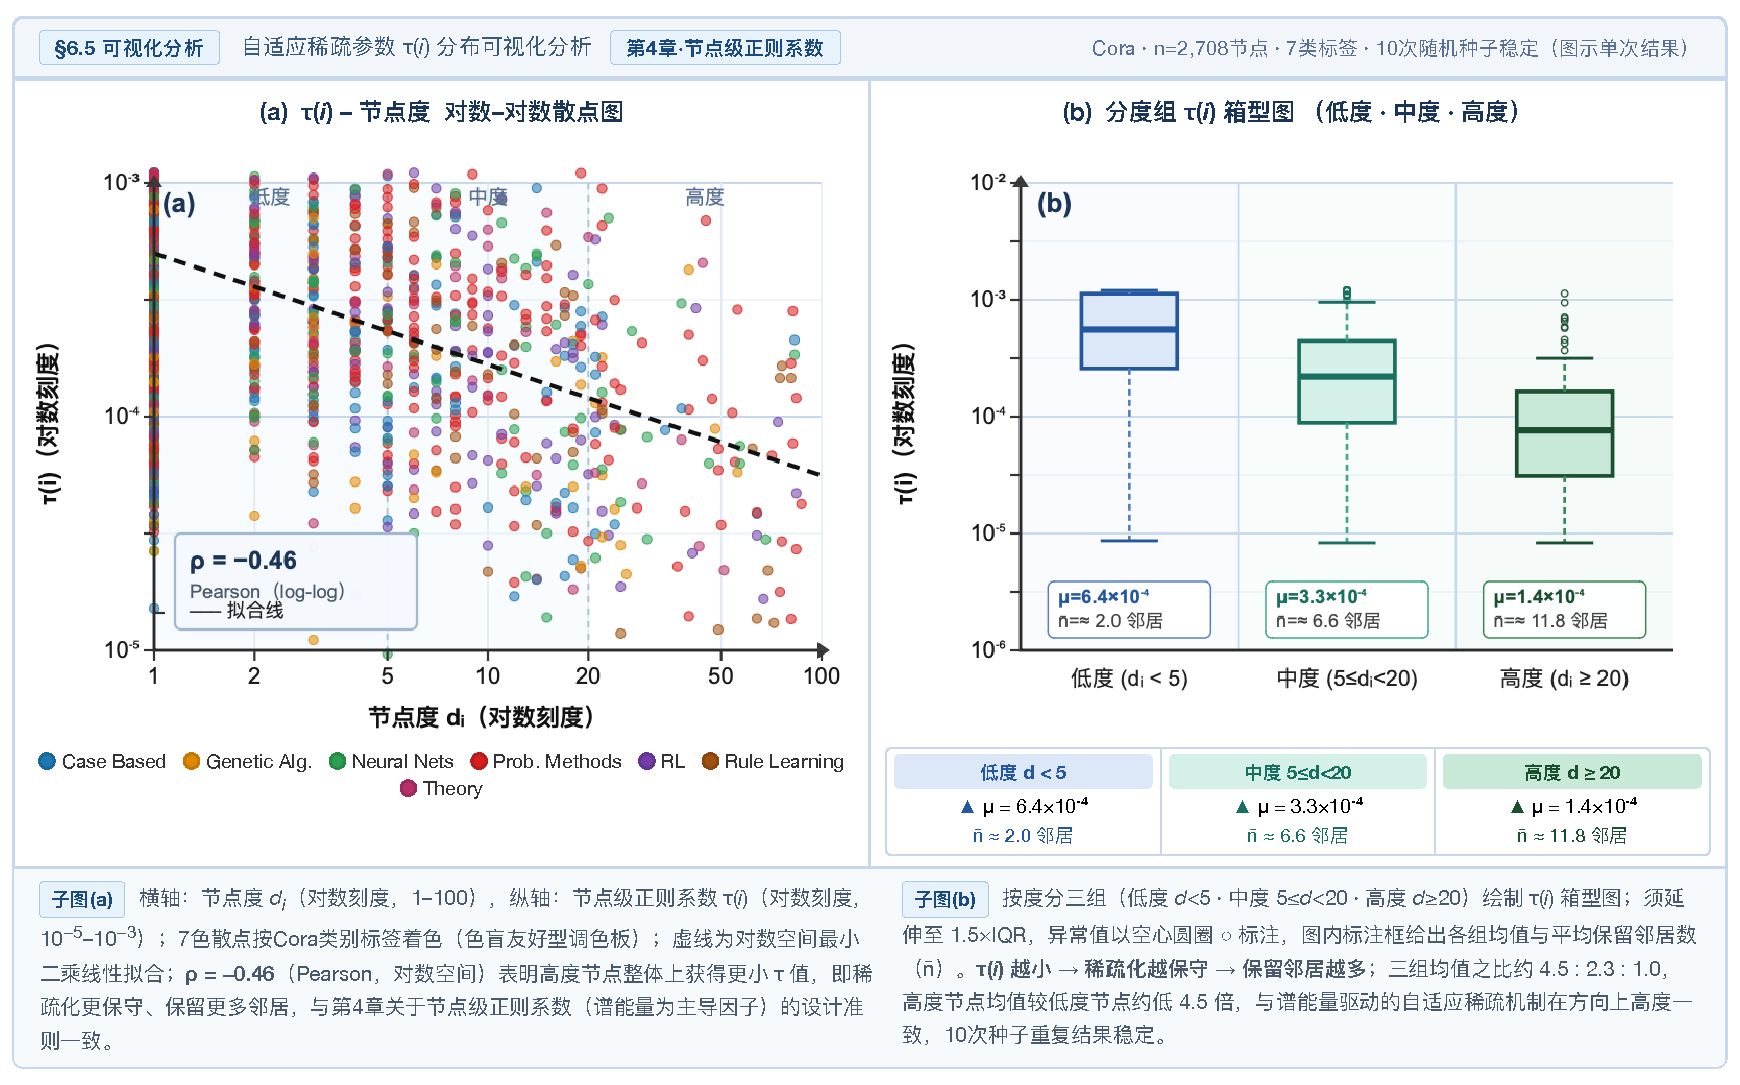
\includegraphics[width=\linewidth]{figures/6-2.pdf}
  \centering
  \vspace{-0.4cm}

  图6.2：$\tau(i)$ 参数分布（Cora）
  枢纽节点集中在低 $\tau$ 区域，
  验证了结构驱动设计方向正确


\end{column}
\end{columns}
\end{frame}

% ==============================================================
% S17  主要贡献与创新点
% ==============================================================
\section{总结与展望}
\setchapternote{第7章}

\begin{frame}{主要贡献与创新点}
  \begin{columns}[T]
    \begin{column}{0.48\textwidth}
      \textbf{\blue{贡献一}}：在 SDGNN 接口内引入节点级自适应稀疏分配
      \begin{itemize}
        \item 以可计算图结构统计量（谱间隙、谱能量、局部图熵、中心性）驱动"哪个节点保留多少邻居"的参数化设计
        \item 将统一稀疏控制问题转化为具体的节点级参数设计问题
        \item 保留单次稀疏矩阵乘推理形式与 $O(n\kbar d)$ 复杂度保证
      \end{itemize}

      \vspace{0.2cm}
      \textbf{\blue{贡献二}}：构建三维自适应参数体系
      \begin{itemize}
        \item \textbf{频率维}：等权节点谱能量（任务无关）
        \item \textbf{节点维}：多因子融合 $\tau(i)$（谱能量+图熵+度中心性+$k$-core）
        \item \textbf{跳距维}：近邻优先分层预算 $k_i^{(l)}$（随跳距递减）
        \item 三个维度在第5章共同进入分层 LARS 求解流程，图结构统计量从解释变量转化为稀疏权重学习的实际调节因素
      \end{itemize}
    \end{column}

    \begin{column}{0.48\textwidth}
      \textbf{\blue{贡献三}}：在统一实验口径下验证精度与效率

      \textbf{精度}（vs.\ SDGNN，Wilcoxon $p<0.05$，全部6个数据集）：
      \begin{itemize}
        \item 引文网络均值 \green{+1.3\%}，结果方差同步下降
        \item 网页图均值 \green{+1.9\%}，复杂拓扑下更优
        \item ogbn-arxiv \green{+0.86\%}，大规模图上有效
      \end{itemize}

      \vspace{0.15cm}
      \textbf{效率}（推理阶段，相对 GCN）：
      \begin{itemize}
        \item 四数据集推理加速 \blue{$8.0\times$}（均值）
        \item ogbn-arxiv 加速 \blue{$14.7\times$}
        \item 峰值显存节省 \blue{74.8\%}
        \item 相对 SDGNN 额外显存增量仅 +41\,MB
      \end{itemize}

      \vspace{0.15cm}
      \begin{alertblock}{方法适用范围}
        \small 教师表示已给定、稀疏权重可离线固化、在线推理需低时延的 SDGNN 式稀疏分解场景
      \end{alertblock}
    \end{column}
  \end{columns}
\end{frame}

% ==============================================================
% S18  局限性、未来工作与致谢
% ==============================================================
\begin{frame}{研究局限与未来展望}
  \begin{columns}[T]
    \begin{column}{0.48\textwidth}
      \textbf{\highlight{研究局限性}}（§\,7.3）
      \begin{enumerate}\setlength{\itemsep}{4pt}
        \item \textbf{启发式近似性质}\\
          $\tau(i)$ 基于代理变量构造，尚未严格刻画与最优稀疏支撑的充要关系；重尾度分布、强异配图上的适用边界待进一步分析
        \item \textbf{静态图假设}\\
          方法适用 transductive 设定，$\Theta^{\mathrm{fixed}}$ 在新节点或边结构变化时未必继续适用；动态场景的稀疏权重维护未系统讨论
        \item \textbf{误差界的条件化性质}\\
          谱相似性分析提供误差\textbf{方向解释}，非对所有图结构最优稀疏性的严格保证
      \end{enumerate}
    \end{column}

    \begin{column}{0.48\textwidth}
      \textbf{\blue{未来研究方向}}（§\,7.4）
      \begin{enumerate}\setlength{\itemsep}{4pt}
        \item \textbf{理论深化}\\
          引入局部谱扰动分析，建立 $\tau(i)$、$k_i^{(l)}$ 与 $\sigma$-谱相似性的可检验关系，将条件化误差解释推进为直接参数设计指导
        \item \textbf{结构可靠性增强}\\
          引入边级可靠性评分（结构相似性+对比学习表征），通过软门控调节 LARS 候选集，联合优化图结构质量与预算分配
        \item \textbf{动态图适配}\\
          设计增量维护机制，局部变化时对受影响节点进行 warm-start 重估；实现分层更新策略（局部微调/部分重训练/全局热启动）
      \end{enumerate}
    \end{column}
  \end{columns}

  \vspace{0.2cm}
  \begin{center}
    \large\textbf{感谢翟铮副教授的悉心指导与北京师范大学文理学院（统计学院）各位老师的支持}\\[0.3cm]
    \LARGE\highlight{欢迎各位评委老师提问与批评指正}
  \end{center}
\end{frame}

\end{document}